\documentclass[conference]{IEEEtran}
\IEEEoverridecommandlockouts

\usepackage{kotex} % review draft only; src/to_english.py removes it
\usepackage{booktabs,multirow,amsmath,graphicx}
\usepackage{cite}
\usepackage[hidelinks]{hyperref}
\usepackage[ruled]{algorithm}
\usepackage[noend]{algpseudocode}
\usepackage{tikz}
\usepackage{pgfplots}

\def\BibTeX{{\rm B\kern-.05em{\sc i\kern-.025em b}\kern-.08em
    T\kern-.1667em\lower.7ex\hbox{E}\kern-.125emX}}

\definecolor{vskeyword}{HTML}{AF00DB}\definecolor{vsfunction}{HTML}{795E26}\definecolor{vsvariable}{HTML}{001080}\definecolor{vsnumber}{HTML}{098658} % VS Code Light+ (Figure 3)
\pgfplotsset{compat=1.18,
 tick label style={font=\scriptsize}, label style={font=\footnotesize},
 legend style={font=\scriptsize, draw=none},
 reference/.style={fill=white, draw=black},
 baseline1/.style={fill=gray!35, draw=black},
 baseline2/.style={fill=gray!60, draw=black},
 baseline3/.style={fill=gray!85, draw=black},
 proposed/.style={fill=blue!12, postaction={pattern=north east lines, pattern color=blue!50}, draw=black},
 proposedlight/.style={fill=white, postaction={pattern=north east lines, pattern color=blue!50}, draw=black},
 variant/.style={fill=gray!25, draw=black},
 referenceline/.style={red!85!black, thick},
 verdictline/.style={gray!70!black, thick},
 refactoryline/.style={orange!90!black, thick},
 brafarline/.style={yellow!70!black, thick},
 mentoredline/.style={green!60!black, thick},
 qwenline/.style={cyan!70!black, thick},
 gptline/.style={blue!80!black, thick},
 toacceptance/.style={fill=green!55!black!55, draw=black},
 forwardstep/.style={fill=green!30, draw=black},
 sidewaysstep/.style={fill=gray!20, draw=black},
 regressstep/.style={fill=red!25, draw=black},
 proposedline/.style={violet, thick}}
\usetikzlibrary{arrows.meta,positioning,fit,calc,backgrounds,patterns}


\title{Trajectory-Supervised Repair for Automated Feedback Generation}

\begin{document}

\maketitle

\begin{abstract}
% 우리는 학생이 내딛는 크기의 걸음을 돌려주는 trajectory-supervised repair 기법 \textsc{ZPDPatch}를 제시한다. 대부분의 기존 Automated Feedback Generation(AFG) 기법은 test suite에 비추어 틀린 제출을 수리한다. 그러나 이런 AFG 기법은 정답 프로그램을 목표로 삼으므로, 수리의 최대 57.8\%는 학생이 두 제출 사이에서 고친 가장 큰 폭을 넘는다. 반면 학생은 한 걸음씩 더 많은 test case를 통과해 가지만, 이렇게 앞으로 나아간 걸음의 최대 95.2\%는 verdict를 바꾸지 않아 verdict로는 드러나지 않는다. 학생 trajectory는 이미 그런 걸음을 담고 있는데, 판정기의 verdict를 받은 뒤 낸 각 제출은 학생이 도움을 받아 닿는 영역인 Zone of Proximal Development 안의 걸음이기 때문이다. \textsc{ZPDPatch}는 틀린 제출마다 test case별 실행 결과로 판정한 같은 학생의 이후 앞으로 나아간 걸음을 짝짓고(Mine), 짝짓는 규칙마다 모델을 학습하며(Train), 검증 프로그램을 함께 가장 많이 수리하는 모델들을 고른다(Select). AtCoder 14개 문제의 버기 프로그램 1,753개에서 \textsc{ZPDPatch}의 수리 가운데 76.7\%는 그 가장 큰 폭 안에 들며, 이는 네 가지 최신 AFG 기법(baseline)보다 최대 81.5\% 더 자주 그렇다. \textsc{ZPDPatch}와 baseline이 모두 수리한 프로그램에서 \textsc{ZPDPatch}의 patch는 최대 60.9\% 작고 학생의 code를 최대 27.6\% 더 많이 남긴다. 또한 \textsc{ZPDPatch}의 수리 가운데 16.3\%는 학습에도 수리에도 쓰지 않은 학생 자신의 accepted 프로그램과 AST가 같아, 어느 baseline보다도 두 배 넘게 많다. 수리하지 못한 프로그램의 9.5\%에서도 \textsc{ZPDPatch}는 학생의 걸음만큼 통과율을 높이는 앞으로 나아간 걸음을 돌려준다.
We present \textsc{ZPDPatch}, a trajectory-supervised repair technique that returns steps of the size students take. Most existing Automated Feedback Generation (AFG) techniques repair a wrong submission against the test suite. However, these AFG techniques aim at a correct program, so up to 57.8\% of their repairs exceed the largest change the student made between two submissions. Students instead pass more test cases step by step, yet up to 95.2\% of these forward steps keep the verdict, which cannot reveal them. Student trajectories already hold such steps, since each submission after the judge's verdict is a step within the student's Zone of Proximal Development, the zone reached with help. \textsc{ZPDPatch} pairs each wrong submission with the student's later forward steps, judged by test-case-wise outcomes (Mine), trains a model per pairing rule (Train), and selects the models that together repair the most validation programs (Select). On 1,753 buggy programs from 14 AtCoder problems, 76.7\% of the repairs of \textsc{ZPDPatch} lie within that largest change, up to 81.5\% more often than for four state-of-the-art AFG techniques (baselines). On the programs that \textsc{ZPDPatch} and a baseline both repair, the patches of \textsc{ZPDPatch} are up to 60.9\% smaller and keep up to 27.6\% more of the student's code. Moreover, 16.3\% of the repairs of \textsc{ZPDPatch} match the abstract syntax tree of the student's own unseen accepted program, over twice as often as for any baseline. On 9.5\% of the programs it does not repair, \textsc{ZPDPatch} still returns forward steps that raise the pass rate as much as students' steps do.
\end{abstract}

\begin{IEEEkeywords}
Automated Program Repair, Automated Feedback Generation, Zone of Proximal Development, Submission Trajectories, Test Oracles
\end{IEEEkeywords}

\section{Introduction}
\label{sec:introduction}

% Automated Feedback Generation(AFG)은 프로그래밍 과목의 각 학생에게 틀린 제출에 대한 개인화된 피드백을 준다~\cite{keuning2018systematic}. 학생은 같은 과제를 여러 번 제출하며, online judge나 autograder가 돌려주는 verdict와 테스트 결과는 무엇을 수리해야 할지 거의 알려 주지 않는다. 그래서 대부분의 기존 AFG 기법은 Automated Program Repair(APR)~\cite{gazzola2017automatic,monperrus2018automatic}로 틀린 제출을 수리하고 개인화된 patch를 돌려주며, 이 patch는 학생에게 막힌 곳에서 앞으로 나아갈 길을 보여 준다~\cite{wang2018search,gulwani2018automated,hu2019re,choi2025automated}. 그러나 일반 APR 도구가 주로 고쳐 온 개발자 프로그램은 일부 test case만 실패하는 반면 학생 프로그램은 여러 결함을 포함하는 경우가 많아, 최근의 code LLM을 포함한 일반 APR 도구를 그대로 적용하면 학생 프로그램을 최대 약 30\%만 수리한다~\cite{yi2017feasibility,gu2025can}. 그래서 AFG 기법은 일반 APR과 따로, 학생 프로그램에 맞춘 수리 기법으로 발전해 왔다. 이 기법들은 test suite를 oracle로 삼아~\cite{barr2014oracle} 모든 test case를 통과하는 첫 후보 프로그램을 돌려준다.
Automated Feedback Generation (AFG) gives each student in a programming course personalized feedback on a wrong submission~\cite{keuning2018systematic}. Students submit the same assignment many times, and the verdict and test results that an online judge or autograder returns rarely tell them what to repair. Most existing AFG techniques therefore repair the wrong submission with Automated Program Repair (APR)~\cite{gazzola2017automatic,monperrus2018automatic} and return the personalized patch, which shows a student a way forward from where they are stuck~\cite{wang2018search,gulwani2018automated,hu2019re,choi2025automated}. However, developer programs, which general APR tools usually repair, fail only a few test cases, whereas student programs often contain multiple faults, so general APR tools, including a recent code language model, repaired at most about 30\% of student programs when applied as is~\cite{yi2017feasibility,gu2025can}. AFG techniques have therefore developed their own repair, tailored to student programs, apart from general APR. They take the test suite as the oracle~\cite{barr2014oracle} and return the first candidate program that passes every test case.

% 틀린 제출을 수리하는 AFG 기법은 수리를 무엇 쪽으로 이끄는지에 따라 두 부류로 나뉜다. Reference-driven 기법은 수리를 같은 문제의 reference program 쪽으로~\cite{gulwani2018automated,hu2019re,choi2025automated,wang2018search,choi2021automated,xie2024brafar} 이끌고, Model-driven 기법은 언어 모델이 학습한 정답 코드 쪽으로~\cite{joshi2023repair,heo2023referent,zhang2024pydex,phung2023generating,liu2024fastfixer,yang2024cref,zhao2026peer,orvalho2025counterexample,dai2026learner} 이끈다. 두 부류의 기법은 버기 프로그램의 수리율을 높여 왔으며~\cite{koutcheme2024benchmarking}, 최근 기법은 최소 수정 patch(minimal-edit patch)도 지향한다~\cite{choi2025automated,dai2026learner}.
AFG techniques that repair a wrong submission fall into two groups by what they steer a repair toward. Reference-driven techniques steer it toward reference programs of the same problem~\cite{gulwani2018automated,hu2019re,choi2025automated,wang2018search,choi2021automated,xie2024brafar}, and Model-driven techniques toward the correct code a language model has learned~\cite{joshi2023repair,heo2023referent,zhang2024pydex,phung2023generating,liu2024fastfixer,yang2024cref,zhao2026peer,orvalho2025counterexample,dai2026learner}. Both groups have raised the repair rate on buggy programs~\cite{koutcheme2024benchmarking}, and recent techniques also aim for minimal-edit patches~\cite{choi2025automated,dai2026learner}.

% 그러나 우리가 관찰한 바는 기존 AFG 기법이 학생의 reach 밖의 patch를 자주 돌려준다는 것이다. 이 연구에서 우리는 이런 수리를 \emph{solution-supervised}라 부르는데, 이 수리는 reference program이나 모델이 학습한 코드 같은 정답 프로그램을 목표로 삼을 뿐, 학생이 그 문제에 낸 제출의 순서인 trajectory에서 내디뎌 온 걸음은 보지 않기 때문이다. 학습자의 과제는 (1) 혼자 할 수 있는 영역, (2) 도움을 받아야 할 수 있는 영역, (3) 도움을 받아도 아직 할 수 없는 영역으로 나뉘며, (2) 영역을 Zone of Proximal Development(ZPD)라 한다~\cite{cole1978mind}. 피드백은 학생이 따라갈 수 있는 만큼만, 즉 학습자의 ZPD 안에서만 도움이 된다~\cite{narciss2008feedback,aleven2000limitations}. 학생은 한 번에 정답 프로그램에 이르지 않으며, 평균 통과율은 첫 틀린 제출의 68.9\%에서 마지막 틀린 제출의 77.1\%로 오른다. 반면 최신 AFG 기법들~\cite{hu2019re,xie2024brafar,choi2025automated,dai2026learner}의 수리 가운데 최대 57.8\%는 학생이 판정기의 도움을 받아 그 문제에서 내디딘 가장 큰 걸음을 넘는다. 그 결과 학생은 자신의 ZPD를 넘는 patch를 자주 받으며, 이런 patch는 학생이 스스로 따라가기 어려울 수 있다.
However, our observation is that existing AFG techniques often return a patch beyond the student's reach. In this work, we call such repair \emph{solution-supervised}, as it targets a correct program, a reference program or code a model has learned, regardless of the steps the student has taken in their trajectory, the sequence of submissions to the problem. A learner's tasks fall into three zones, those the learner can do (1) alone, (2) only with help, and (3) not yet even with help, and zone (2) is the Zone of Proximal Development (ZPD)~\cite{cole1978mind}. Feedback helps only as far as the student can follow it~\cite{narciss2008feedback,aleven2000limitations}, that is, within the learner's ZPD. Students do not reach a correct program at once, and their mean pass rate rises from 68.9\% at their first wrong submission to 77.1\% at their last. In contrast, up to 57.8\% of the repairs of state-of-the-art AFG techniques~\cite{hu2019re,xie2024brafar,choi2025automated,dai2026learner} exceed the largest step the student took on the problem with the judge's help. Consequently, students often receive a patch beyond their ZPD, which they may find hard to follow on their own.

% 이 논문에서 우리는 학생의 ZPD 안의 걸음을 돌려주는 trajectory-supervised repair 기법 \textsc{ZPDPatch}를 제시한다. 우리의 통찰은 학생 trajectory가 이미 그런 걸음을 담고 있다는 것으로, 학생이 판정기의 verdict를 받은 뒤 내는 제출은 도움을 받아 도달한 걸음이며 \emph{trajectory-supervised repair}는 이 걸음들로부터 학습한다. 그러려면 각 학생의 trajectory에서 어느 이후 제출이 앞으로 나아간 걸음인지 가려내야 하며, 그러지 않으면 모델이 학생이 뒤로 물러난 걸음까지 학습하게 된다. 핵심 도전과제는 이 걸음을 찾는 것으로, acceptance 전 학생들의 앞으로 나아간 걸음 가운데 최대 95.2\%가 verdict를 바꾸지 않아 verdict만으로는 찾을 수 없다(Section~\ref{sec:limitation}). 이 도전과제를 해결하기 위해 \textsc{ZPDPatch}는 Mine, Train, Select의 세 단계로 동작한다. Mine 단계는 세 target 규칙에 따라 버기 프로그램을 같은 학생의 accepted 제출(Answer), verdict가 덜 심각한 다음 제출(Strict), 또는 test case별 실행 결과에서 어느 test case도 나빠지지 않고 적어도 하나가 나아진 다음 제출(Progress)과 짝짓는다. Train 단계는 규칙과 seed마다 adapter 하나를 학습하고, Select 단계는 검증 버기 프로그램을 함께 가장 많이 수리하는 checkpoint 셋을 고른다. 수리 시점에 \textsc{ZPDPatch}는 현재 제출만 읽으며, 어느 후보도 통과하지 않으면 같은 비교로 찾은 앞으로 나아간 걸음을 돌려준다. 기존 AFG 기법이 정답 프로그램을 목표로 삼는 것과 달리, \textsc{ZPDPatch}는 정답이든 부분 정답이든 학생의 ZPD 안의 patch를 목표로 삼는다.
In this paper, we present \textsc{ZPDPatch}, a trajectory-supervised repair technique that returns a step within the student's ZPD. Our insight is that student trajectories already contain such steps, since the submission a student makes after the judge's verdict is a step reached with help, and \emph{trajectory-supervised repair} learns from these steps. Learning from them requires telling which later submissions in each student's trajectory are forward steps, or the model would also learn the steps students took back. A key challenge lies in finding these steps, since up to 95.2\% of the students' forward steps before acceptance leave the verdict unchanged, so the verdict alone cannot find them (Section~\ref{sec:limitation}). To address this challenge, \textsc{ZPDPatch} operates in three stages, Mine, Train, and Select. The Mine stage pairs a buggy program, under three target rules, with the same student's accepted submission (Answer), next submission with a less severe verdict (Strict), or next submission whose test-case-wise outcomes are worse on no test case and better on at least one (Progress). The Train stage trains one adapter per rule and seed, and the Select stage chooses the three checkpoints that together repair the most validation buggy programs. At repair time, \textsc{ZPDPatch} reads only the current submission and, if no candidate passes, returns the forward step found by the same comparison. Unlike existing AFG techniques, which aim at a correct program, \textsc{ZPDPatch} aims at a patch within the student's ZPD, whether the patch is correct or only partially correct.

% 실험 결과는 \textsc{ZPDPatch}가 돌려주는 걸음이 학생 자신의 걸음을 닮았음을 보여 준다. 우리는 AtCoder 14개 문제의 Python 버기 프로그램 1,753개에서 \textsc{ZPDPatch}를 네 가지 최신 AFG 기법~\cite{hu2019re,xie2024brafar,choi2025automated,dai2026learner}(baseline)과 비교했다. \textsc{ZPDPatch}가 수리한 프로그램 가운데 76.7\%는 학생이 그 문제에서 내디딘 가장 큰 걸음(그 학생의 \emph{demonstrated reach}) 안에 들며, 이 비율은 baseline보다 최대 81.5\% 높다. \textsc{ZPDPatch}와 baseline이 모두 수리한 버기 프로그램에서 \textsc{ZPDPatch}의 patch는 크기가 최대 60.9\% 작고 학생의 code를 최대 27.6\% 더 많이 남긴다. 또한 \textsc{ZPDPatch}가 수리한 프로그램의 16.3\%는 학습에도 수리에도 쓰지 않은 학생 자신의 accepted 프로그램과 AST가 같아, 어느 baseline보다도 두 배 넘게 많다. \textsc{ZPDPatch}가 수리하지 못한 버기 프로그램의 9.5\%에서는, 학생 자신의 앞으로 나아간 걸음처럼 통과율을 중앙값 12.5 포인트 높이는 앞으로 나아간 걸음을 돌려준다.
Experimental results demonstrate that the steps \textsc{ZPDPatch} returns resemble the students' own steps. We compared \textsc{ZPDPatch} with four state-of-the-art AFG techniques~\cite{hu2019re,xie2024brafar,choi2025automated,dai2026learner} as baselines on 1,753 Python buggy programs from 14 AtCoder problems. Of the programs \textsc{ZPDPatch} repairs, 76.7\% lie within the largest step the student took on the problem (their \emph{demonstrated reach}), a share up to 81.5\% larger than that of the baselines. On the buggy programs that both \textsc{ZPDPatch} and a baseline repair, the patches of \textsc{ZPDPatch} are up to 60.9\% smaller and keep up to 27.6\% more of the student's code. Moreover, 16.3\% of the programs \textsc{ZPDPatch} repairs have the same abstract syntax tree as the student's own accepted program, which neither training nor repair sees, more than twice as often as for any baseline. On 9.5\% of the buggy programs that \textsc{ZPDPatch} does not repair, it returns a forward step that raises the pass rate by a median of 12.5 points, as the students' own forward steps do.

% \noindent\textbf{Contributions.} 우리의 기여를 아래와 같이 요약한다:
\noindent\textbf{Contributions.} We summarize our contributions below:
\begin{itemize}
% \item \textbf{Observation.} 우리는 기존 AFG 기법이 학생의 ZPD를 넘어 학생이 아직 닿지 않는 영역의 patch를 자주 돌려주며, verdict만 보는 oracle은 acceptance 전 학생들의 앞으로 나아간 걸음 대부분을 가린다는 것을 보인다(Section~\ref{sec:limitation}).
\item \textbf{Observation.} We show that existing AFG techniques often return patches beyond the student's ZPD, in the zone the student cannot yet reach, and that a verdict-only oracle hides most of the students' forward steps before acceptance (Section~\ref{sec:limitation}).
% \item \textbf{New technique.} 우리는 학생의 ZPD 안의 걸음을 돌려주는 trajectory-supervised repair 기법 \textsc{ZPDPatch}를 제시한다. \textsc{ZPDPatch}의 특화된 알고리즘은 verdict가 바뀌지 않아 가려진 앞으로 나아간 걸음을 reference program 없이 mine하되, 뒤로 물러났다 되돌아온 제출을 세지 않도록 test case별 실행 결과를 retained trajectory의 마지막 제출과 비교하고, target 규칙과 seed마다 adapter를 학습하며, 검증 버기 프로그램을 함께 가장 많이 수리하는 checkpoint들을 고른다.
\item \textbf{New technique.} We present \textsc{ZPDPatch}, a trajectory-supervised repair technique that returns steps within the student's ZPD. The specialized algorithm of \textsc{ZPDPatch} mines, without a reference program, the forward steps an unchanged verdict hides, comparing test-case-wise outcomes with the last submission of the retained trajectory so that returning after a regression does not count, trains one adapter per target rule and seed, and selects the checkpoints that together repair the most validation buggy programs.
% \item \textbf{Evaluation.} 우리는 네 가지 최신 AFG 기법과 비교해 \textsc{ZPDPatch}의 수리 가운데 학생의 reach 안에 드는 비율이 더 크고, \textsc{ZPDPatch}의 patch가 더 작고 학생의 code를 더 많이 남기며 학생 자신의 accepted 프로그램과 AST가 같은 경우가 더 많음을 보인다. 우리는 \textsc{ZPDPatch}를 \url{https://anonymous.4open.science/r/zpdpatch}에 공개한다.
\item \textbf{Evaluation.} We show that, against four state-of-the-art AFG techniques, a larger share of the repairs of \textsc{ZPDPatch} lies within the student's reach, and the patches of \textsc{ZPDPatch} are smaller, keep more of the student's code, and more often have the same abstract syntax tree as the student's own accepted program. We make \textsc{ZPDPatch} publicly available at \url{https://anonymous.4open.science/r/zpdpatch}.
\end{itemize}


\section{Preliminaries}
\label{sec:preliminaries}

\subsection{Automated Feedback Generation for Programming Assignments}
\label{sec:formulation}

% 프로그래밍 과제를 위한 수리 기법은 학생의 틀린 제출, 즉 \emph{buggy program} \(b\)를 그 문제의 test suite \(T\)에 있는 모든 test case를 통과하는 프로그램으로 바꾼다. 기존 기법은 \(b\)와 \(T\)에 더해 부류에 따라 다른 입력을 쓴다. Reference-driven 기법은 같은 문제의 \emph{reference program} 집합 \(R\), 즉 다른 학생들의 정답 제출로 \(b\)를 고치며 problem description은 쓰지 않는다~\cite{gulwani2018automated,wang2018search,hu2019re,choi2025automated}. Model-driven 기법은 problem description \(\mathit{desc}\)를 언어 모델에 주며, 일부는 다른 학생의 제출 \(R\)을 예시로 더한다~\cite{heo2023referent,zhao2026peer,dai2026learner}.
Repair techniques for programming assignments turn a student's wrong submission, the \emph{buggy program} \(b\), into a program that passes every test case of the problem's test suite \(T\). Besides \(b\) and \(T\), existing techniques use different inputs by group. Reference-driven techniques repair \(b\) from the set \(R\) of \emph{reference programs} of the same problem, i.e., correct submissions of other students, and do not use the problem description~\cite{gulwani2018automated,wang2018search,hu2019re,choi2025automated}. Model-driven techniques give the problem description \(\mathit{desc}\) to a language model, and some add the submissions \(R\) of other students as examples~\cite{heo2023referent,zhao2026peer,dai2026learner}.

\begin{algorithm}[h]
\caption{Generic repair procedure}
\label{alg:generic}
\footnotesize
\begin{algorithmic}[1]
\item[\textbf{Input:}] Buggy program ($b$), Problem description ($\mathit{desc}$), Reference programs ($R$), Test suite ($T$)
\item[\textbf{Output:}] Patch ($p$)
\Procedure{Repair}{$b, \mathit{desc}, R, T$}
\For{$r\in\mathsf{Top}_k(R,b)$} \Comment{the $k$ closest to $b$ by $\mathsf{sim}$, e.g., $k=1$}
 \If{Reference-driven}
  \State $A\gets\mathsf{Align}(b,r)$ \Comment{blocks of $b$ to those of $r$}
  \State $p\gets\mathsf{Edit}(b,r,A)$ \Comment{differing blocks from $r$}
 \Else \Comment{Model-driven}
  \State $p\gets M(\mathsf{Prompt}(\mathit{desc},b,r))$
 \EndIf
 \State $T_{\mathit{pass}}\gets\textsc{Execute}(p,T)$
 \If{$T_{\mathit{pass}}=1$} \State \Return $p$ \EndIf
\EndFor
\State \Return $b$
\EndProcedure
\end{algorithmic}
\end{algorithm}

% Algorithm~\ref{alg:generic}은 이런 기존 기법의 일반 수리 절차를 기술한다. 2번째 줄은 \(R\) 가운데 \(b\)와의 유사도 \(\mathsf{sim}(b,r)\)가 가장 높은 \(k\)개의 reference program \(r\)을 차례로 취한다. 가장 가까운 하나만 쓰는 기법도 있고(\(k=1\))~\cite{hu2019re,zhao2026peer}, 여러 개를 쓰는 기법도 있다~\cite{wang2018search,dai2026learner}. reference program을 쓰지 않는 기법에서 \(R\)은 빈 프로그램 하나만 담는다. 두 부류는 \(r\)로 후보 \(p\)를 만드는 방식만 다르다. Reference-driven 기법은 \(b\)의 블록을 \(r\)의 블록에 대응시키고(4번째 줄), 대응하는 블록과 다른 \(b\)의 블록을 \(r\)의 것으로 바꾼다(5번째 줄). Model-driven 기법은 \(\mathit{desc}\), \(b\), \(r\)로 prompt를 만들어 언어 모델 \(M\)이 생성한 프로그램을 후보로 삼는다(7번째 줄). 8--10번째 줄은 후보를 \(T\)에서 실행하는데, \textsc{Execute}는 \(p\)가 통과하는 \(T\)의 test case 비율, 즉 \emph{pass rate} \(T_{\mathit{pass}}\)를 돌려주며, \(T_{\mathit{pass}}=1\)이면, 즉 모든 test case를 통과하면 그 후보를 즉시 돌려준다. 어느 후보도 통과하지 않으면 11번째 줄은 \(b\)를 그대로 돌려준다. 어느 부류든 수리는 solution-supervised이며, 학생 자신의 trajectory를 참조하지 않고 고른 정답 프로그램을 향한다.
Algorithm~\ref{alg:generic} describes the generic repair procedure of these techniques. Line~2 takes in turn the \(k\) reference programs \(r\) of \(R\) with the highest similarity \(\mathsf{sim}(b,r)\) to \(b\). Some techniques use only the closest one (\(k=1\))~\cite{hu2019re,zhao2026peer}, and others several~\cite{wang2018search,dai2026learner}. For a technique that uses no reference program, \(R\) holds a single empty program. The two groups differ only in how they build a candidate \(p\) from \(r\). A Reference-driven technique maps the blocks of \(b\) to those of \(r\) (line~4) and replaces each block of \(b\) that differs from its counterpart with that of \(r\) (line~5). A Model-driven technique builds a prompt from \(\mathit{desc}\), \(b\), and \(r\), and takes the program its language model \(M\) generates as the candidate (line~7). Lines~8--10 execute the candidate on \(T\), where \textsc{Execute} returns the \emph{pass rate} \(T_{\mathit{pass}}\) of \(p\), the fraction of the test cases of \(T\) that it passes, and return the candidate as soon as \(T_{\mathit{pass}}=1\), that is, as soon as it passes every test case. If no candidate passes, line~11 returns \(b\) itself. In either group, repair is solution-supervised, heading for a correct program chosen without reference to the student's own trajectory.

\subsection{Limitation of Solution-Supervised Repair}
\label{sec:limitation}

% 우리의 핵심 관찰은 solution-supervised repair가 학생이 내디딘 어떤 걸음보다도 큰 patch를 자주 돌려준다는 것이다. 학생은 제출마다 판정기의 verdict를 받고 다음 제출에서 프로그램을 고치며, 우리는 이 고침을 \emph{step}이라 부른다. step의 크기 \(\mathrm{ted}^{\dagger}\)는 두 프로그램의 Abstract Syntax Tree(AST) 사이의 Tree Edit Distance(TED)로, 코드가 같으면 0이고 변경이 많을수록 \(\infty\)까지 커지는 값이며, 학생의 Zone of Proximal Development(ZPD)에 대한 우리의 관측 가능한 지표다. patch의 크기도 \(b\)로부터의 \(\mathrm{ted}^{\dagger}\)로 재고, 학생이 한 문제에서 내디딘 가장 큰 걸음을 \emph{demonstrated reach}라 부른다.
Our key observation is that solution-supervised repair often returns a patch larger than any step the student has taken. A student receives the judge's verdict on every submission and revises the program in the next one, and we call this revision a \emph{step}. The size \(\mathrm{ted}^{\dagger}\) of a step is the Tree Edit Distance (TED) between the Abstract Syntax Trees (ASTs) of the two programs, ranging from 0 for identical code to \(\infty\) as the change grows, and is our observable measure of the student's Zone of Proximal Development (ZPD). The size of a patch is likewise its \(\mathrm{ted}^{\dagger}\) from \(b\), and we call the largest step a student took on a problem their \emph{demonstrated reach}.

\begin{table}[h]
\caption{Baselines' patches against the students' own steps}
\label{tab:reach}
\centering\scriptsize
\setlength{\tabcolsep}{2.5pt}
\begin{tabular}{@{}l||r|rrr|rrr|rrr@{}}
\toprule
 & & \multicolumn{3}{c|}{TED (\%)} & \multicolumn{3}{c|}{Tokens (\%)} & \multicolumn{3}{c}{Lines (\%)} \\
\cmidrule(lr){3-5}\cmidrule(lr){6-8}\cmidrule(l){9-11}
 & Fixes & $<$ & $=$ & $>$ & $<$ & $=$ & $>$ & $<$ & $=$ & $>$ \\
\midrule
% rows:reach
\textsc{Refactory} & 952 & 29.2 & 4.8 & 66.0 & 73.9 & 6.3 & 19.7 & 83.7 & 9.1 & 7.1 \\
\textsc{Brafar} & 962 & 27.9 & 3.7 & 68.4 & 79.4 & 3.3 & 17.3 & 82.3 & 10.5 & 7.2 \\
\textsc{Mentored} & 705 & 37.3 & 9.2 & 53.5 & 63.4 & 9.4 & 27.2 & 73.5 & 15.5 & 11.1 \\
\textsc{LSGen}\textsubscript{Qwen} & 1,392 & 17.6 & 5.4 & 77.0 & 79.5 & 6.8 & 13.7 & 81.4 & 11.6 & 7.0 \\
\textsc{LSGen}\textsubscript{GPT} & 1,615 & 20.4 & 5.9 & 73.7 & 78.5 & 7.1 & 14.4 & 82.7 & 9.7 & 7.6 \\
% end rows
\bottomrule
\end{tabular}
\end{table}

% 기존 AFG 기법은 정답 프로그램까지를 patch 하나로 건너뛰므로 학생의 걸음보다 큰 patch를 자주 돌려준다. Table~\ref{tab:reach}은 우리의 baseline(Section~\ref{sec:settings})인 부류별 최신 기법들~\cite{hu2019re,xie2024brafar,choi2025automated,dai2026learner}이 마지막 틀린 제출을 수리한 patch(Fixes)마다, 그 TED와 버기 프로그램의 token 및 줄을 남긴 비율을 그 제출에서 accepted 프로그램까지의 학생 걸음의 값과 비교해 작은(\(<\)), 같은(\(=\)), 큰(\(>\)) 경우의 비율로 보인다. accepted 프로그램이 학생에게 한 걸음 거리라 baseline에게 가장 유리한 위치인데도, patch가 학생의 걸음보다 큰 경우가 53.5--77.0\%로 작은 경우의 17.6--37.3\%보다 많았고, token과 줄을 학생의 걸음보다 덜 남긴 경우도 63.4--79.5\%와 73.5--83.7\%였다. 특히 수리의 29.1--57.8\%는 학생의 demonstrated reach마저 넘었다. 그 결과 학생은 자신의 ZPD를 넘는 patch를 자주 받는다.
Existing AFG techniques reach a correct program in one patch and thus often return a patch larger than the student's step. For each patch (Fixes) with which our baselines (Section~\ref{sec:settings}), state-of-the-art techniques of each group~\cite{hu2019re,xie2024brafar,choi2025automated,dai2026learner}, repair the last wrong submission, Table~\ref{tab:reach} compares its TED and the shares of the buggy program's tokens and lines it keeps with those of the student's step from that submission to the accepted program, and shows the shares of the cases where they are smaller (\(<\)), equal (\(=\)), or larger (\(>\)). Although this position, one student step away from the accepted program, is the most favorable to the baselines, 53.5--77.0\% of their patches were larger than the student's step, against 17.6--37.3\% smaller, and 63.4--79.5\% and 73.5--83.7\% kept fewer of the buggy program's tokens and lines, respectively, than the student's step. In particular, 29.1--57.8\% of the repairs exceeded even the student's demonstrated reach. Consequently, students often receive a patch beyond their ZPD.

\begin{figure}[h]
\centering
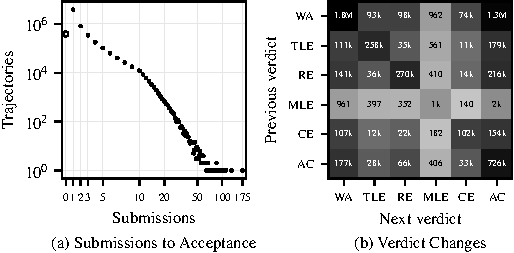
\includegraphics[width=\columnwidth]{output/fig-attempts.pdf}%
\caption{AtCoder submissions in Project CodeNet}
\label{fig:attempts}
\end{figure}

% 반면 학생은 한 번에 정답 프로그램에 이르지 않는다. Figure~\ref{fig:attempts}은 Project CodeNet~\cite{puri2021codenet}에 있는 AtCoder 문제 1,519개 전체의 제출 11,961,031개 전체에서, 각 trajectory가 몇 번째 제출에서 처음 accepted를 받는지(a)와, 연속한 두 제출 사이에서 verdict, 즉 Wrong Answer(WA), Time Limit Exceeded(TLE), Runtime Error(RE), Memory Limit Exceeded(MLE), Compile Error(CE), Accepted(AC)가 어떻게 바뀌는지(b)를 보인다. Figure~\ref{fig:attempts}-(a)에서 첫 제출이 틀린 trajectory 2,018,970개 가운데 59.7\%는 세 번째 이후에야 accepted를 받았거나 끝내 받지 못했다(0). verdict만 받고 내디딘 이 중간 걸음들이 학생이 자신의 ZPD 안에서 실제로 닿은 걸음이다. 그러나 Figure~\ref{fig:attempts}-(b)에서 틀린 제출에서 틀린 제출로 간 걸음 3,180,805개의 76.1\%는 verdict가 그대로여서(대각선 칸), 이 중간 걸음이 정답 쪽으로 나아갔는지는 verdict에 드러나지 않았다. 그렇다고 이 걸음들이 제자리걸음이었던 것은 아니다. 우리 벤치마크의 trajectory 1,753개(Section~\ref{sec:settings})에서 학생의 평균 pass rate는 첫 틀린 제출의 68.9\%에서 마지막 틀린 제출의 77.1\%로 8.2\%p 올랐고, 틀린 제출 사이의 걸음을 test case별 결과로 나누면 27.6\%는 앞으로 나아갔고(verdict가 덜 심각해졌거나, verdict가 같고 어떤 test case도 나빠지지 않고 하나 이상이 나아짐), 32.3\%는 모든 test case가 그대로였으며, 40.0\%는 verdict나 test case를 나쁘게 만들며 물러섰다. 앞으로 나아간 걸음의 95.2\%는 verdict가 그대로였으므로, 같은 verdict로는 걸음이 test case를 나아지게 했든, 그대로 두었든, 나빠지게 했든 가를 수 없다. verdict보다 세밀한 통과한 test case의 수로도 충분하지 않은데, 몇 개를 통과했는지만 셀 뿐, 어떤 test case를 통과했는지도, 실패한 test case가 어떤 verdict를 받았는지도 보지 않기 때문이다. 예를 들어, test case별 통과 여부가 \((1,0,0)\)인 WA 제출에서 \((1,1,0)\)인 WA 제출, \((0,1,1)\)인 WA 제출, 그리고 \((1,1,0)\)이지만 셋째 test case에서 RE가 난 RE 제출로 가는 세 걸음은 모두 통과 수가 하나 늘지만, 앞으로 나아간 것은 첫째뿐이다. 둘째는 통과하던 test case를 깨뜨렸고, 셋째는 verdict가 RE로 나빠졌다. 실제로 pass rate가 오른 걸음의 29.5\%는 verdict나 어떤 test case의 결과를 나쁘게 만들었다.
In contrast, students do not reach a correct program at once. Figure~\ref{fig:attempts} shows, for all 11,961,031 submissions to all 1,519 AtCoder problems of Project CodeNet~\cite{puri2021codenet}, the submission at which each trajectory is first accepted (a) and how the verdict, Wrong Answer (WA), Time Limit Exceeded (TLE), Runtime Error (RE), Memory Limit Exceeded (MLE), Compile Error (CE), or Accepted (AC), changes between consecutive submissions (b). In Figure~\ref{fig:attempts}-(a), 59.7\% of the 2,018,970 trajectories whose first submission was wrong were accepted only at the third submission or later or never (0). These intermediate steps, taken with only the verdict, are the steps the students actually reached within their ZPD. In Figure~\ref{fig:attempts}-(b), however, 76.1\% of the 3,180,805 steps from one wrong submission to the next kept the verdict (the diagonal cells), so whether these intermediate steps moved toward a correct program did not show in the verdict. Yet these steps were not standstills. In the 1,753 trajectories of our benchmark (Section~\ref{sec:settings}), the students' mean pass rate rose by 8.2 points from 68.9\% at the first wrong submission to 77.1\% at the last, and by their test-case outcomes, 27.6\% of the steps between wrong submissions moved forward (to a less severe verdict, or to the same verdict with no test case worse and at least one better), 32.3\% left every test case as it was, and 40.0\% regressed, worsening the verdict or a test case. Since 95.2\% of the forward steps kept the verdict, the same verdict cannot tell whether a step made test cases better, left them as they were, or made them worse. The number of passed test cases, finer than the verdict, is not enough either, because it counts how many test cases pass but neither which ones nor which verdict the failing ones receive. For example, from a WA submission that passes the test cases as \((1,0,0)\), the steps to a WA submission passing \((1,1,0)\), to a WA submission passing \((0,1,1)\), and to an RE submission passing \((1,1,0)\) with a Runtime Error on the third test case all pass one more test case, yet only the first moves forward. The second breaks a test case already passing, and the third worsens the verdict to RE. Indeed, 29.5\% of the steps that raised the pass rate worsened the verdict or the outcome of some test case.

% 이 논문은 학생의 ZPD를 넘는 patch 대신, 정답 프로그램에 이르지 못하더라도 학생을 앞으로 나아가게 하는, 학생의 ZPD~\cite{cole1978mind} 안의 걸음을 돌려주는 것을 목표로 한다. 따라서 우리는 Algorithm~\ref{alg:generic}의 언어 모델 \(M\)을 학생이 자신의 ZPD 안에서 실제로 닿은 이후 제출 쪽으로 학습시키고, 무엇을 반환할지는 test suite가 정하게 한다. 그러나 틀린 제출 사이의 걸음 가운데 40.0\%는 물러섰으므로, 이를 거르지 않고 학습하면 모델이 물러서는 걸음까지 배운다. 이 때문에 핵심 도전과제는 앞으로 나아간 걸음을 reference program 없이 verdict와 test case별 실행 결과를 함께 보아 가려내는 것이다.
The goal of this paper is to return, instead of a patch beyond the student's ZPD, a step within the student's ZPD~\cite{cole1978mind}, one that moves the student forward even when it does not reach a correct program. We therefore train the language model \(M\) of Algorithm~\ref{alg:generic} toward the student's own later submissions, which the student actually reached within their ZPD, and let the test suite decide what is returned. However, 40.0\% of the steps between wrong submissions regressed, so a model trained on them unfiltered would also learn to regress. The key challenge is thus to tell forward steps apart, without reference programs, by both the verdict and the test-case outcomes.


\section{Our Approach}
\label{sec:approach}

\subsection{Overview}
\label{sec:construct}

\begin{figure}[h]
\centering
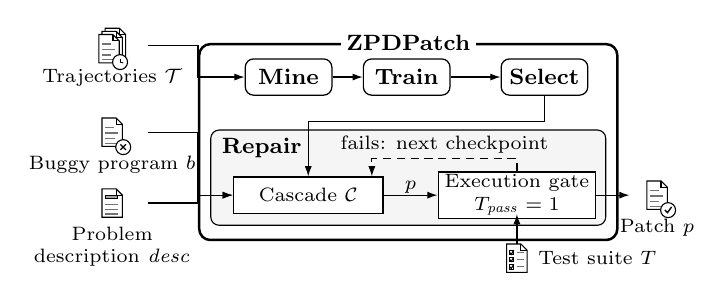
\begin{tikzpicture}[font=\scriptsize, >={Latex[length=1.3mm,width=0.9mm]}, line width=0.45pt,
 stage/.style={draw, rounded corners=3pt, minimum width=11mm, minimum height=4.6mm, align=center,
               font=\footnotesize\bfseries, fill=white, inner sep=1pt},
 sub/.style={draw, minimum width=19mm, minimum height=4.6mm, inner sep=1pt, align=center, fill=white},
 lbl/.style={font=\scriptsize, inner sep=0.5pt},
 item/.style={align=center, inner sep=0.4pt, font=\scriptsize},
 icsheet/.pic={\draw[fill=white, line width=0.4pt]
               (-1.3mm,-1.8mm) -- (-1.3mm,1.8mm) -- (0.5mm,1.8mm) -- (1.3mm,1.0mm) -- (1.3mm,-1.8mm) -- cycle;
             \draw[line width=0.4pt] (0.5mm,1.8mm) -- (0.5mm,1.0mm) -- (1.3mm,1.0mm);},
 iccode/.pic={\pic{icsheet};
            \foreach \y/\a/\b in {0.6/-0.9/0.2, -0.1/-0.9/0.7, -0.8/-0.9/0.3, -1.4/-0.9/0.8}
              \draw[line width=0.42pt, black!55] (\a mm,\y mm) -- (\b mm,\y mm);},
 icstack/.pic={\pic at (0.4mm,0.4mm) {icsheet}; \pic at (0mm,0mm) {icsheet}; \pic at (-0.4mm,-0.4mm) {iccode};},
 icbadge/.pic={\draw[fill=white, line width=0.4pt] (0,0) circle (0.95mm);},
 icclock/.pic={\pic{icbadge}; \draw[line width=0.35pt] (0,0) -- (0,0.45mm); \draw[line width=0.35pt] (0,0) -- (0.4mm,-0.1mm);},
 iccross/.pic={\pic{icbadge}; \draw[line width=0.45pt] (-0.35mm,-0.35mm) -- (0.35mm,0.35mm) (-0.35mm,0.35mm) -- (0.35mm,-0.35mm);},
 ictick/.pic={\pic{icbadge}; \draw[line width=0.5pt] (-0.4mm,0.02mm) -- (-0.08mm,-0.32mm) -- (0.44mm,0.4mm);},
 ichead/.pic={\pic{icsheet};
            \draw[fill=black!35, line width=0pt] (-0.9mm,0.55mm) rectangle (0.7mm,1.0mm);
            \foreach \y in {-0.2,-0.8,-1.4} \draw[line width=0.42pt, black!55] (-0.9mm,\y mm) -- (0.7mm,\y mm);},
 iclist/.pic={\pic{icsheet};
            \foreach \y in {0.7,-0.2,-1.1} {
              \draw[line width=0.33pt] (-0.95mm,\y mm-0.28mm) rectangle (-0.45mm,\y mm+0.28mm);
              \draw[line width=0.4pt] (-0.9mm,\y mm) -- (-0.72mm,\y mm-0.22mm) -- (-0.4mm,\y mm+0.32mm);
              \draw[line width=0.42pt, black!55] (-0.05mm,\y mm) -- (0.85mm,\y mm);}},
 iclog/.pic={\pic{icsheet};
            \draw[line width=0.45pt] (-0.95mm,0.75mm) -- (-0.75mm,0.5mm) -- (-0.4mm,1.05mm);
            \draw[line width=0.45pt] (-0.95mm,-0.45mm) -- (-0.4mm,0.1mm) (-0.95mm,0.1mm) -- (-0.4mm,-0.45mm);
            \draw[line width=0.45pt] (-0.95mm,-1.5mm) -- (-0.75mm,-1.75mm) -- (-0.4mm,-1.2mm);
            \foreach \y in {0.75,-0.2,-1.35} \draw[line width=0.42pt, black!55] (-0.05mm,\y mm) -- (0.85mm,\y mm);},
 icruler/.pic={\draw[fill=white, line width=0.4pt] (-1.5mm,-0.9mm) rectangle (1.5mm,0.9mm);
            \foreach \x in {-1.0,-0.5,0,0.5,1.0} \draw[line width=0.35pt] (\x mm,0.9mm) -- (\x mm,0.25mm);
            \draw[line width=0.35pt] (-1.5mm,-0.35mm) -- (1.5mm,-0.35mm);},
 ictraj/.pic={\pic{icstack}; \pic at (1.0mm,-2.1mm) {icclock};},
 icbuggy/.pic={\pic{iccode}; \pic at (1.4mm,-1.9mm) {iccross};},
 icfixed/.pic={\pic{iccode}; \pic at (1.4mm,-1.9mm) {ictick};}]

 % ---- bands
 \node[stage] (mine)  at (2.80,  5mm) {Mine};
 \node[stage] (train) at (4.30,  5mm) {Train};
 \node[stage] (sel)   at (6.05,  5mm) {Select};
 \node[sub] (gen)  at (3.05, -10mm) {Cascade $\mathcal C$};
 \node[sub, minimum width=20mm] (gate) at (5.70, -10mm) {Execution gate\\$T_{\mathit{pass}}=1$};
 \node[font=\footnotesize\bfseries, inner sep=0.4pt] (dtitle) at (2.46, -4mm) {Repair};
 \begin{scope}[on background layer]
   \node[draw, rounded corners=3pt, fit=(dtitle)(gen)(gate), inner xsep=1.2mm, inner ysep=0.8mm, fill=black!4] (dep) {};
 \end{scope}
 \begin{scope}[on background layer]
   \node[draw, line width=0.9pt, rounded corners=4pt, fit=(mine)(sel)(dep), inner xsep=1.4mm, inner ysep=1.8mm] (tool) {};
 \end{scope}
 \node[fill=white, inner xsep=2pt, inner ysep=0.4pt, font=\footnotesize\bfseries] at (tool.north) {\textsc{ZPDPatch}};

 % ---- one icon per named item
 \pic at (0.56,  9mm) {ictraj};   \node[item, anchor=north] at (0.56,  6.2mm) {Trajectories $\mathcal T$};
 \pic at (0.56, -2mm) {icbuggy};  \node[item, anchor=north] at (0.56, -4.8mm) {Buggy program $b$};
 \pic at (0.56,-11mm) {ichead};   \node[item, anchor=north] at (0.56,-13.8mm) {Problem\\description $\mathit{desc}$};
 \pic at (5.70,-18mm) {iclist};  \node[item, anchor=west] at (5.95,-18mm) {Test suite $T$};
 \pic at (7.48,-10mm) {icfixed}; \node[item, anchor=north] at (7.48,-12.8mm) {Patch $p$};

 % ---- wires
 \coordinate (bus) at (1.65, 0);
 \coordinate (corr) at (0, -0.6mm);
 \draw[->] (1.01,  9mm) -- (1.65,  9mm) |- (mine.west);
 \draw[->] (1.01, -2mm) -- (1.65, -2mm) |- (gen.west);
 \draw[->] (1.01,-11mm) -- (1.65,-11mm) |- (gen.west);
 \draw[->] (5.70,-16.2mm) -- (5.70,-12.4mm);
 \draw[->] (mine) -- (train);
 \draw[->] (train) -- (sel);
 \draw[->] (sel.south) -- (sel.south |- corr) -- (gen.north |- corr) -- (gen.north);
 \draw[->] (gen) -- node[lbl, above] {$p$} (gate);
 \draw[->] (gate.east) -- (7.13, -10mm);
 \draw[->, densely dashed] (gate.north) -- ++(0,1.6mm) -| node[lbl, pos=0.25, above=0.5mm] {fails: next checkpoint} ([xshift=-1.5mm]gen.north east);
\end{tikzpicture}
\caption{Overview of \textsc{ZPDPatch}}
\label{fig:overview}
\end{figure}

% Figure~\ref{fig:overview}은 \textsc{ZPDPatch}의 전체 입출력과 흐름을 보인다. \textsc{ZPDPatch}는 학생의 버기 프로그램 \(b\), problem description \(\mathit{desc}\), test suite \(T\)를 받아 patch \(p\)를 돌려주며, 학습을 위해 과목의 지난 제출 기록인 trajectory \(\mathcal T\)를 받는다. 오프라인에서 \textsc{ZPDPatch}는 코퍼스마다 한 번, Mine, Train, Select의 세 단계로 \(\mathcal T\)를 처리한다. Mine 단계는 학습 쌍을, Train 단계는 언어 모델을 그 쌍으로 fine-tune한 \emph{checkpoint}들을 만들고, Select 단계는 그 가운데 학습에서 제외한 버기 프로그램을 함께 가장 많이 수리하는 checkpoint 셋을 순서대로 묶은 \emph{cascade} \(\mathcal C\)를 고른다. Repair에서는 학생이 판정기가 거부하는 프로그램 \(b\)를 제출하면, cascade의 checkpoint가 차례로 \(\mathit{desc}\)와 그 현재 제출만 읽고 후보 patch \(p\)를 만든다. Execution gate는 \(p\)를 \(T\)에서 실행해 모든 test case를 통과하면(\(T_{\mathit{pass}}=1\)) \(p\)를 돌려주고, 그렇지 않으면 다음 checkpoint로 넘어간다.
Figure~\ref{fig:overview} shows the overall inputs, outputs, and flow of \textsc{ZPDPatch}. \textsc{ZPDPatch} takes a student's buggy program \(b\), the problem description \(\mathit{desc}\), and the test suite \(T\) and returns a patch \(p\), and for training it takes trajectories \(\mathcal T\), a course's past submission records. Offline, once per corpus, \textsc{ZPDPatch} processes \(\mathcal T\) in three stages, Mine, Train, and Select. Mine builds training pairs, Train fine-tunes a language model on them into \emph{checkpoints}, and Select picks the \emph{cascade} \(\mathcal C\), three ordered checkpoints that together repair the most buggy programs held out of training. In Repair, when a student submits a program \(b\) that the judge rejects, the checkpoints of the cascade in turn read only \(\mathit{desc}\) and that current submission and produce a candidate patch \(p\). The execution gate runs \(p\) on \(T\) and returns \(p\) if it passes every test case (\(T_{\mathit{pass}}=1\)), and otherwise moves on to the next checkpoint.

\begin{algorithm}[h]
\caption{\textsc{ZPDPatch}}
\label{alg:construct}
\footnotesize
\begin{algorithmic}[1]
\item[\textbf{Input:}] Buggy program ($b$), Problem description ($\mathit{desc}$), Test suite ($T$), Trajectories ($\mathcal T$)
\item[\textbf{Output:}] Patch ($p$)
\Procedure{ZPDPatch}{$b, \mathit{desc}, T, \mathcal T$}
\State $\langle D_A, D_S, D_P, \Theta\rangle\gets\langle\emptyset,\emptyset,\emptyset,\emptyset\rangle$ \Comment{Training pairs, checkpoints}
\Statex\hspace{\algorithmicindent}/* Step 1. Mine stage */
\For{$\tau=[b_1,\ldots,b_n,c]\in\mathcal T$} \Comment{Buggy $b_i$, Correct $c$}
 \State $D_A\gets D_A\cup\{([b_i],c)\mid i\le n\}$ \Comment{Pair each $b_i$ with $c$}
 \For{$\rho\in\{S,P\}$} \Comment{$\rho\in\{\mathit{Strict},\mathit{Progress}\}$}
  \State $\tau_R\gets[b_1]$ \Comment{Retained trajectory}
  \For{$s\in[b_2,\ldots,b_n,c]$}
   \If{$\mathsf{Improves}_{\rho}(\tau_R,s)$} \Comment{Check if $s$ moves forward}
    \State $D_\rho\gets D_\rho\cup\{(\tau_R,s)\}$; $\tau_R\gets \tau_R\mathbin{\|}[s]$
   \EndIf
  \EndFor
 \EndFor
\EndFor
\Statex\hspace{\algorithmicindent}/* Step 2. Train stage */
\For{$(\rho,\sigma)\in\{A,S,P\}\times[1,\eta_\sigma]$} \Comment{$\eta_\sigma$ seeds per rule}
 \State $\Theta\gets\Theta\cup\{\mathsf{Train}(D_\rho,\sigma)\}$ \Comment{Fine-tune $M$ with seed $\sigma$}
\EndFor
\Statex\hspace{\algorithmicindent}/* Step 3. Select stage */
\For{$\theta\in\Theta$}
 \State $F_{\theta}\gets\mathsf{Validate}(\theta,\mathcal T)$ \Comment{Run on held-out buggy programs}
\EndFor
\State $\mathcal C\gets\mathsf{Select}(\{F_{\theta}\}_{\theta\in\Theta},\eta_{\mathcal C})$ \Comment{Cascade of $\eta_{\mathcal C}$ checkpoints}
\Statex\hspace{\algorithmicindent}/* Repair */
\State $\langle p^*,T_{\mathit{pass}}^*\rangle\gets\langle b,\textsc{Execute}(b,T)\rangle$
\For{$\theta\in\mathcal C$}
 \State $p\gets M_\theta(\mathsf{Prompt}(\mathit{desc},b))$
 \State $T_{\mathit{pass}}\gets\textsc{Execute}(p,T)$
 \If{$T_{\mathit{pass}}=1$} \State \Return $p$ \EndIf
 \If{$\mathsf{Improves}_P([b],p)\land T_{\mathit{pass}}>T_{\mathit{pass}}^*$}
  \State $\langle p^*,T_{\mathit{pass}}^*\rangle\gets\langle p,T_{\mathit{pass}}\rangle$ \Comment{Keep the best forward step}
 \EndIf
\EndFor
\State \Return $p^*$ \Comment{$p^*=b$ if no candidate moves forward}
\EndProcedure
\end{algorithmic}
\end{algorithm}

% Algorithm~\ref{alg:construct}은 \textsc{ZPDPatch}의 절차를 기술한다. Section~\ref{sec:formulation}의 Algorithm~\ref{alg:generic}이 수리할 때마다 다른 학생의 correct program \(R\)을 참조하는 것과 달리, Algorithm~\ref{alg:construct}은 수리 전에 오프라인에서 학습 코퍼스의 trajectory \(\mathcal T\)로 학습하고, 수리할 때는 그 결과인 checkpoint만 쓴다. \(\mathcal T\)의 \emph{trajectory} \(\tau=[b_1,\ldots,b_n,c]\)는 한 학생이 한 문제에 낸 제출들을 시간순으로 늘어놓은 것으로, 버기 프로그램 \(b_1,\ldots,b_n\) 뒤에 첫 accepted 제출인 correct program \(c\)로 끝난다. 3--9번째 줄의 Mine은 Section~\ref{sec:limitation}의 도전과제대로 verdict와 test case별 결과를 함께 보아 앞으로 나아간 걸음을 학습 쌍으로 모으고, 10--11번째 줄의 Train은 그 쌍으로 Algorithm~\ref{alg:generic}의 언어 모델 \(M\)을 fine-tune한 checkpoint를 만들며, 12--14번째 줄의 Select는 그 가운데 cascade \(\mathcal C\)를 고른다(Section~\ref{sec:mine}--\ref{sec:select}). 15--23번째 줄은 학습에 쓰지 않은 학생의 새 제출 \(b\)를 수리하며, Algorithm~\ref{alg:generic}의 Model-driven 경로와 세 가지가 다르다. \(R\)의 reference program 대신 \(\mathcal C\)의 checkpoint \(\theta\)를 차례로 순회하고(16번째 줄), prompt에는 \(\mathit{desc}\)와 \(b\)만 담으며(17번째 줄), 어느 후보도 통과하지 않으면 \(b\) 대신, \(\mathsf{Improves}_P\)로 판정한 \(b\)로부터의 앞으로 나아간 걸음 가운데 pass rate가 \(b\)보다 높으면서 가장 높은 것을 돌려준다(21--23번째 줄). 통과하는 첫 후보를 돌려주므로 \(\mathcal C\)의 순서는 수리 여부가 아니라 어떤 patch를 돌려줄지를 정한다.
Algorithm~\ref{alg:construct} gives the procedure of \textsc{ZPDPatch}. Unlike Algorithm~\ref{alg:generic} of Section~\ref{sec:formulation}, which consults the reference programs \(R\), correct programs of other students, at every repair, Algorithm~\ref{alg:construct} learns offline from the trajectories \(\mathcal T\) of the training corpus before any repair and uses only the resulting checkpoints at repair time. A \emph{trajectory} \(\tau=[b_1,\ldots,b_n,c]\) of \(\mathcal T\) orders one student's submissions to a problem chronologically, the buggy programs \(b_1,\ldots,b_n\) followed by the first accepted one, the correct program \(c\). Mine at lines~3--9 collects the forward steps as training pairs, reading both the verdict and the test-case outcomes as the challenge of Section~\ref{sec:limitation} requires, Train at lines~10--11 fine-tunes the language model \(M\) of Algorithm~\ref{alg:generic} on them into checkpoints, and Select at lines~12--14 chooses the cascade \(\mathcal C\) among them (Sections~\ref{sec:mine}--\ref{sec:select}). Lines~15--23 repair the new submission \(b\) of a student not used in training and differ from the Model-driven branch of Algorithm~\ref{alg:generic} in three ways. They iterate over the checkpoints \(\theta\) of \(\mathcal C\) instead of over the reference programs of \(R\) (line~16), prompt with \(\mathit{desc}\) and \(b\) only (line~17), and, if no candidate passes, return instead of \(b\) the forward step from \(b\), judged by \(\mathsf{Improves}_P\), with the highest pass rate above that of \(b\) (lines~21--23). Because the first passing candidate is returned, the order of \(\mathcal C\) decides which patch is returned, not whether one is found.

\begin{figure*}[t]
\centering\scriptsize
\setlength{\fboxsep}{0pt}
\begin{minipage}[t]{0.315\textwidth}
\begin{tabular}[t]{@{}r@{~}l@{}}
{\color{black!55}13} & \makebox[4.3cm][l]{\texttt{\textcolor{vskeyword}{if}~\textcolor{vsvariable}{S}[\textcolor{vsnumber}{0}]~==~\textcolor{vsnumber}{0}:}} \\
{\color{black!55}14} & \makebox[4.3cm][l]{\texttt{~~~~\textcolor{vsfunction}{print}(-\textcolor{vsnumber}{1})}} \\
{\color{black!55}15} & \makebox[4.3cm][l]{\texttt{~~~~\textcolor{vsfunction}{exit}()}} \\
{\color{black!55}16} & \makebox[4.3cm][l]{\texttt{\textcolor{vskeyword}{if}~\textcolor{vsvariable}{S}[\textcolor{vsnumber}{0}]~==~-\textcolor{vsnumber}{1}:}} \\
{\color{black!55}17} & \colorbox{black!10}{\makebox[4.3cm][l]{\strut\texttt{~~~~\textcolor{vsvariable}{S}[-\textcolor{vsnumber}{1}]~=~\textcolor{vsnumber}{1}}}} \\
\end{tabular}
\end{minipage}\hfill
\begin{minipage}[t]{0.315\textwidth}
\begin{tabular}[t]{@{}r@{~}l@{}}
{\color{black!55}13} & \makebox[4.3cm][l]{\texttt{\textcolor{vskeyword}{if}~\textcolor{vsvariable}{S}[\textcolor{vsnumber}{0}]~==~\textcolor{vsnumber}{0}:}} \\
{\color{black!55}14} & \makebox[4.3cm][l]{\texttt{~~~~\textcolor{vsfunction}{print}(-\textcolor{vsnumber}{1})}} \\
{\color{black!55}15} & \makebox[4.3cm][l]{\texttt{~~~~\textcolor{vsfunction}{exit}()}} \\
{\color{black!55}16} & \makebox[4.3cm][l]{\texttt{\textcolor{vskeyword}{if}~\textcolor{vsvariable}{S}[\textcolor{vsnumber}{0}]~==~-\textcolor{vsnumber}{1}:}} \\
{\color{black!55}17} & \colorbox{black!10}{\makebox[4.3cm][l]{\strut\texttt{~~~~\textcolor{vsvariable}{S}[\textcolor{vsnumber}{0}]~=~\textcolor{vsnumber}{1}}}} \\
\end{tabular}
\end{minipage}\hfill
\begin{minipage}[t]{0.315\textwidth}
\begin{tabular}[t]{@{}r@{~}l@{}}
{\color{black!55}13} & \makebox[4.3cm][l]{\texttt{\textcolor{vskeyword}{if}~\textcolor{vsvariable}{S}[\textcolor{vsnumber}{0}]~==~\textcolor{vsnumber}{0}:}} \\
{\color{black!55}14} & \colorbox{black!10}{\makebox[4.3cm][l]{\strut\texttt{~~~~\textcolor{vskeyword}{if}~\textcolor{vsvariable}{N}~!=~\textcolor{vsnumber}{1}:}}} \\
{\color{black!55}15} & \makebox[4.3cm][l]{\texttt{~~~~~~~~\textcolor{vsfunction}{print}(-\textcolor{vsnumber}{1})}} \\
{\color{black!55}16} & \makebox[4.3cm][l]{\texttt{~~~~~~~~\textcolor{vsfunction}{exit}()}} \\
{\color{black!55}17} & \makebox[4.3cm][l]{\texttt{\textcolor{vskeyword}{if}~\textcolor{vsvariable}{S}[\textcolor{vsnumber}{0}]~==~-\textcolor{vsnumber}{1}:}} \\
{\color{black!55}18} & \colorbox{black!10}{\makebox[4.3cm][l]{\strut\texttt{~~~~\textcolor{vskeyword}{if}~\textcolor{vsvariable}{N}~!=~\textcolor{vsnumber}{1}:}}} \\
{\color{black!55}19} & \makebox[4.3cm][l]{\texttt{~~~~~~~~\textcolor{vsvariable}{S}[\textcolor{vsnumber}{0}]~=~\textcolor{vsnumber}{1}}} \\
{\color{black!55}20} & \colorbox{black!10}{\makebox[4.3cm][l]{\strut\texttt{~~~~\textcolor{vskeyword}{else}:}}} \\
{\color{black!55}21} & \colorbox{black!10}{\makebox[4.3cm][l]{\strut\texttt{~~~~~~~~\textcolor{vsvariable}{S}[\textcolor{vsnumber}{0}]~=~\textcolor{vsnumber}{0}}}} \\
\end{tabular}
\end{minipage}\par\smallskip
\begin{minipage}[t]{0.315\textwidth}\centering (a) Buggy program $b_1$ (61.1\% passed)\end{minipage}\hfill
\begin{minipage}[t]{0.315\textwidth}\centering (b) Next buggy program $b_2$ (88.9\% passed)\end{minipage}\hfill
\begin{minipage}[t]{0.315\textwidth}\centering (c) Correct program $c$\end{minipage}
\caption{Running example (p02761)}
\label{fig:example}
\end{figure*}

\subsection{Mine}
\label{sec:mine}

% Mine 단계는 학습 trajectory에서 학습 쌍을 만든다(3--9번째 줄). 각 쌍은 버기 프로그램, 또는 그때까지 앞으로 나아간 제출들을, 학생이 그 뒤에 실제로 낸 제출과 짝지으며, 어떤 이후 제출을 target으로 삼을지는 세 target 규칙이 정한다. Answer는 accepted 제출인 correct program을, Strict는 verdict가 덜 심각해진 다음 제출을, Progress는 verdict와 test case별 결과로 판정해 앞으로 나아간 다음 제출을 target으로 삼는다. Answer는 각 버기 프로그램을 단독으로 correct program \(c\)와 짝짓지만(4번째 줄), Strict와 Progress는 제출이 앞으로 나아갔는지를 판정해야 한다.
The Mine stage builds training pairs from the training trajectories (lines~3--9). Each pair matches a buggy program, or the submissions that have moved forward up to it, with a later submission the student actually made, and three target rules decide which later submission becomes the target. Answer targets the accepted submission, the correct program, Strict the next submission with a less severe verdict, and Progress the next submission that moved forward as judged by the verdict and the test-case outcomes. Answer pairs each buggy program, on its own, with the correct program \(c\) (line~4), whereas Strict and Progress must judge whether a submission moved forward.

% 이를 위해 우리는 프로그램이 실행의 어느 단계까지 갔는지로 verdict에 순서를 매긴다. severity 함수 \(\mathrm{sev}\)는 컴파일되지 않는 Compile Error(CE)에 4, 실행 중 멈추는 Runtime Error(RE)에 3, 실행되지만 시간이나 메모리 제한을 넘는 Time or Memory Limit Exceeded(TLE/MLE)에 2, 제한 안에 끝나지만 출력이 틀린 Wrong Answer(WA)에 1, Accepted(AC)에 0을 준다. trajectory의 모든 제출 \(s\)에 대해, \(v(s)\)는 판정기가 \(s\) 전체에 내린 verdict(예: WA)이고, \(o(s)\)는 \(s\)를 \(T\)의 test case마다 다시 실행한 결과(예: 첫 test case는 AC, 둘째는 WA)를 그 test case에 대응시킨 것이며, \(\mathrm{sev}\)는 둘 모두에 똑같이 적용된다.
To this end, we order verdicts by how far a program gets through execution. The severity function \(\mathrm{sev}\) assigns 4 to Compile Error (CE), for a program that does not compile, 3 to Runtime Error (RE), for one that stops during execution, 2 to Time or Memory Limit Exceeded (TLE/MLE), for one that runs but exceeds a time or memory limit, 1 to Wrong Answer (WA), for one that ends within the limits with a wrong output, and 0 to Accepted (AC). For every submission \(s\) of a trajectory, \(v(s)\) is the verdict the judge gave to \(s\) as a whole (e.g., WA), \(o(s)\) maps each test case of \(T\) to the outcome of re-executing \(s\) on it (e.g., AC on the first test case and WA on the second), and \(\mathrm{sev}\) applies alike to both.

% Strict와 Progress는 \(\tau\)에서 앞으로 나아간 것으로 판정된 제출만 남긴 \emph{retained trajectory} \(\tau_R\)을 유지하고, 이후 제출 \(s\)를 \(\tau_R\)의 마지막 제출 \(s'=\tau_R[-1]\)과 비교한다. \(s\)가 앞으로 나아간 것으로 판정되면 \(\tau_R\)에 덧붙여져 다음 비교의 \(s'\)이 된다. 어느 test case에서도 \(s\)의 결과가 \(s'\)의 결과보다 나쁘지 않고 적어도 하나에서 더 좋으면, 즉 \(o(s)\)가 \(o(s')\)를 Pareto 지배하면 \(o(s)\prec o(s')\)로 쓴다:
Strict and Progress keep the \emph{retained trajectory} \(\tau_R\), the subsequence of \(\tau\) that retains only the submissions judged to have moved forward, and compare each later submission \(s\) with the last submission \(s'=\tau_R[-1]\) of \(\tau_R\). If \(s\) is judged to have moved forward, it is appended to \(\tau_R\) and becomes \(s'\) for the next comparison. We write \(o(s)\prec o(s')\) when the outcome of \(s\) is no worse than that of \(s'\) on any test case and better on at least one, i.e., when \(o(s)\) Pareto-dominates \(o(s')\):
\[
\begin{aligned}
o(s)\prec o(s')\iff{}&\forall t\in T:\mathrm{sev}(o(s)(t))\le\mathrm{sev}(o(s')(t))\\
&\land\ \exists t\in T:\mathrm{sev}(o(s)(t))<\mathrm{sev}(o(s')(t)).
\end{aligned}
\]
% 그러면 두 규칙의 술어는 다음과 같다:
The predicates of the two rules are then:
\begin{equation}
\begin{aligned}
\mathsf{Improves}_S(\tau_R,s)&\iff \mathrm{sev}(v(s))<\mathrm{sev}(v(s')),\\
\mathsf{Improves}_P(\tau_R,s)&\iff \mathsf{Improves}_S(\tau_R,s)\\
 &\quad\lor\ \bigl(v(s)=v(s')\land o(s)\prec o(s')\bigr).
\end{aligned}
\label{eq:progress}
\end{equation}
% 즉 Progress는 verdict가 그대로여도 어느 test case도 나빠지지 않고 하나 이상 나아지면 앞으로 나아간 것으로 보아, verdict에 가려진 진전까지 가려낸다.
Progress thus counts a step that keeps the verdict as forward if no test case gets worse and at least one improves, telling apart even the progress the verdict hides.

% 두 규칙은 \(\tau_R=[b_1]\)에서 시작해, 이후의 각 제출 \(s\)에 술어가 성립할 때만 \((\tau_R,s)\)를 낸 뒤 \(s\)를 \(\tau_R\)에 덧붙인다(5--9번째 줄). Figure~\ref{fig:example}은 이 차이를 한 trajectory \([b_1,b_2,c]\)에서 보인다. \(b_2\)(Figure~\ref{fig:example}-(b))는 \(b_1\)(Figure~\ref{fig:example}-(a))의 verdict WA를 그대로 두지만, 어떤 test case도 나빠지지 않고 pass rate를 61.1\%에서 88.9\%로 높인다. 그래서 verdict만 보는 Strict는 \(b_2\)를 앞으로 나아간 걸음으로 보지 못해 Answer처럼 \(b_1\)을 \(c\)(Figure~\ref{fig:example}-(c))와 짝짓고, 그 target은 \(b_1\)에서 Tree Edit Distance(TED) 22만큼 떨어져 있다. 반면 Progress는 \(([b_1],b_2)\)와 \(([b_1,b_2],c)\)를 내어, 학생이 실제로 내디딘 TED 3의 걸음을 학습 쌍으로 삼는다. 실제로 Progress는 Strict보다 Seen 학습 쌍을 26.2\% 더 많이 내는데, 그 21,416개 쌍 가운데 4,443개(20.7\%)가 verdict는 그대로이면서 test case별 결과가 나아진 걸음이기 때문이다.
Both rules start with \(\tau_R=[b_1]\) and, for each later submission \(s\), emit \((\tau_R,s)\) and append \(s\) to \(\tau_R\) only when the predicate holds (lines~5--9). Figure~\ref{fig:example} shows the difference on one trajectory \([b_1,b_2,c]\). \(b_2\) (Figure~\ref{fig:example}-(b)) keeps the WA verdict of \(b_1\) (Figure~\ref{fig:example}-(a)) but raises the pass rate from 61.1\% to 88.9\% with no test case worse. Strict, which reads only the verdict, therefore does not see \(b_2\) as a forward step and, like Answer, pairs \(b_1\) with \(c\) (Figure~\ref{fig:example}-(c)), a target at a Tree Edit Distance (TED) of 22 from \(b_1\). In contrast, Progress emits \(([b_1],b_2)\) and \(([b_1,b_2],c)\), taking as a training pair the step of TED 3 the student actually took. Indeed, Progress yields 26.2\% more Seen training pairs than Strict, because 4,443 (20.7\%) of its 21,416 pairs are steps whose verdict stays the same while their test-case outcomes improve.

% 각 제출을 바로 앞 제출이 아니라 \(s'\)과 비교하는 것은, WA에서 RE로 물러선 뒤 WA로 돌아오는 것이 앞으로 나아간 것으로 세어지지 않게 하기 위해서이며, 세 규칙은 Section~\ref{sec:rq-ablation}에서 비교한다.
Each submission is compared with \(s'\) rather than with the immediately preceding submission, so that returning to WA after regressing from WA to RE does not count as moving forward, and Section~\ref{sec:rq-ablation} compares the three rules.

\subsection{Train}
\label{sec:train}
% Train 단계의 목표는 각 target 규칙의 걸음을 언어 모델 \(M\)에 가르치되, 규칙 간 차이가 target에서만 오도록 모델과 최적화를 같게 유지하는 것이다(10--11번째 줄). 11번째 줄에서 \(\mathsf{Train}\)은 규칙 \(\rho\)의 학습 쌍 \(D_\rho\)와 seed \(\sigma\) 하나로 adapter \(\theta\)를 학습해 \(\Theta\)에 더한다. adapter는 \(M\)의 가중치를 그대로 둔 채 덧붙여 학습하는 작은 파라미터이며, 이 adapter가 곧 checkpoint다.
The goal of the Train stage is to teach the language model \(M\) the steps of each target rule while keeping the model and optimization the same across rules, so that the rules differ only in their targets (lines~10--11). At line~11, \(\mathsf{Train}\) learns an adapter \(\theta\) on the training pairs \(D_\rho\) of rule \(\rho\) with one seed \(\sigma\) and adds it to \(\Theta\). An adapter is a small set of parameters trained on top of \(M\) while its weights stay frozen, and this adapter is the checkpoint.

% 학습 쌍 \((\tau_R,s)\)마다, prompt \(q=\mathsf{Prompt}(\mathit{desc},\tau_R)\)는 시간·메모리 제한을 포함한 problem description \(\mathit{desc}\)와 \(\tau_R\)의 제출들을 담는다. \(\tau_R\)은 Answer에서는 버기 프로그램 하나이고, Strict와 Progress에서는 retained trajectory다. 각 제출에는 소스 코드, verdict, 재실행에서 통과한 test case의 수와 실패한 test case별 결과, 앞 제출과 비교한 Abstract Syntax Tree(AST) 변경 요약이 붙고, prompt는 완전한 프로그램을 출력하라는 지시로 끝난다. target은 \(s\)의 소스 코드이며, 수리할 때의 prompt \(\mathsf{Prompt}(\mathit{desc},b)\)는 \(\tau_R=[b]\)인 경우다. 형식적으로, \(\mathsf{Train}\)은 다음을 최소화하는 \(\theta\)를 찾는다:
For each training pair \((\tau_R,s)\), the prompt \(q=\mathsf{Prompt}(\mathit{desc},\tau_R)\) holds the problem description \(\mathit{desc}\), including its time and memory limits, and the submissions of \(\tau_R\). \(\tau_R\) is a single buggy program for Answer and the retained trajectory for Strict and Progress. Each submission comes with its source code, its verdict, the number of test cases it passes on re-execution and the outcomes of those it fails, and a summary of its Abstract Syntax Tree (AST) changes from the previous submission, and the prompt ends with a request for a complete program. The target is the source code of \(s\), and the prompt \(\mathsf{Prompt}(\mathit{desc},b)\) at repair time is the case \(\tau_R=[b]\). Formally, \(\mathsf{Train}\) finds the \(\theta\) that minimizes:
\[
 \mathcal L_\rho(\theta)=-\frac{1}{N_\rho}\sum_{(\tau_R,s)\in D_\rho}\sum_{j=1}^{|s|}\log M_\theta\bigl(y_j\mid q,y_{<j}\bigr),
\]
% 여기서 \(M_\theta\)는 adapter \(\theta\)를 단 \(M\)이고, \(y_j\)는 \(s\)의 \(j\)번째 token이며, \(N_\rho\)는 \(D_\rho\)의 target token 수다. prompt는 규칙도 patch 크기도 밝히지 않으므로, adapter가 얼마나 바꾸는지는 오직 \(D_\rho\)의 target에서 온다.
where \(M_\theta\) is \(M\) with the adapter \(\theta\), \(y_j\) is the \(j\)-th token of \(s\), and \(N_\rho\) is the number of target tokens in \(D_\rho\). Because the prompt names neither the rule nor a patch size, how much an adapter changes comes from the targets of \(D_\rho\) alone.

% 우리는 규칙마다 별도의 adapter를 학습한다. 같은 버기 프로그램이 \(D_A\)에서는 correct program \(c\)와, \(D_P\)에서는 다음에 앞으로 나아간 제출과 짝지어질 수 있으므로, 섞인 규칙으로 학습한 한 모델은 같은 prompt에 서로 다른 target을 받게 되고, prompt에 규칙을 밝히면 수리 전에 규칙을 골라야 하게 된다. 별도의 adapter는 둘 다 피하고, Select가 실행된 검증 수리로 checkpoint를 고르게 한다. 모든 규칙과 seed는 같은 \(M\)과 학습 설정을 쓰며, 그 어느 것도 우리 데이터에서 조정하지 않았다. \(M\), 즉 base model로는 한 과목이 GPU 한 장에서 실행할 수 있을 만큼 작은 공개 code model인 Qwen2.5-Coder-7B-Instruct~\cite{hui2024qwen2}를 쓴다. 각 adapter는 4 bit로 양자화한 \(M\)에 Low-Rank Adaptation(LoRA, rank 16, \(\alpha=32\))을 붙여 QLoRA~\cite{dettmers2023qlora}로 learning rate \(2\times10^{-4}\), batch size 16, 한 epoch 학습하며, 검증 loss로 early stopping을 한다. 규칙마다 seed 셋(\(\eta_\sigma=3\))을 학습하는 이유는, 같은 데이터로 학습해도 seed가 다른 checkpoint는 서로 다른 버기 프로그램을 수리하기 때문이다(Section~\ref{sec:select}).
We train a separate adapter for each rule. The same buggy program can be paired with the correct program \(c\) in \(D_A\) and with the next submission that moved forward in \(D_P\), so one model trained on the mixed rules would receive different targets for the same prompt, and naming the rule in the prompt would require choosing a rule before repairing. Separate adapters avoid both and let Select choose checkpoints by executed validation repairs. Every rule and seed uses the same \(M\) and training settings, none tuned on our data. As \(M\), the base model, we use Qwen2.5-Coder-7B-Instruct~\cite{hui2024qwen2}, an open code model small enough for a course to run on one GPU. Each adapter attaches Low-Rank Adaptation (LoRA, rank 16, \(\alpha=32\)) to \(M\) quantized to 4 bits and is trained with QLoRA~\cite{dettmers2023qlora} at a learning rate of \(2\times10^{-4}\), a batch size of 16, and one epoch, with early stopping on validation loss. We train three seeds per rule (\(\eta_\sigma=3\)) because checkpoints trained on the same data with different seeds repair different buggy programs (Section~\ref{sec:select}).

\subsection{Select}
\label{sec:select}

% Select 단계의 목표는 checkpoint마다 수리하는 버기 프로그램이 다르다는 점을 이용해, 함께 가장 많이 수리하는 checkpoint 몇 개를 cascade로 묶는 것이다(12--14번째 줄). 이를 위해 우리는 \(\mathcal T\)를 학습·검증·테스트로 나눌 때의 검증 분할에서 문제마다 버기 프로그램을 하나씩 뽑아 \(\mathcal B_{\mathit{val}}\)로 두고, cascade를 고르는 데에만 쓴다. 12--13번째 줄에서 \(\mathsf{Validate}\)는 \(\Theta\)의 각 checkpoint \(\theta\)를 \(\mathcal B_{\mathit{val}}\)의 각 버기 프로그램에 한 번씩 실행해, \(\theta\)가 모든 test case를 통과하는 patch로 고친(fixed) 버기 프로그램의 집합 \(F_\theta\subseteq\mathcal B_{\mathit{val}}\)을 기록한다. 14번째 줄에서 \(\mathsf{Select}\)는 각 checkpoint를 따로 순위 매기지 않고, 길이가 \(\eta_{\mathcal C}\)인 cascade 가운데 다음을 최대화하는 조합을 고른다:
The goal of the Select stage is to exploit the fact that different checkpoints repair different buggy programs, bundling the few checkpoints that together repair the most into a cascade (lines~12--14). To this end, we take one buggy program per problem from the validation split made when \(\mathcal T\) is split into training, validation, and test sets, and use these buggy programs \(\mathcal B_{\mathit{val}}\) only to choose the cascade. At lines~12--13, \(\mathsf{Validate}\) runs each checkpoint \(\theta\) of \(\Theta\) once on each buggy program of \(\mathcal B_{\mathit{val}}\) and records the set \(F_\theta\subseteq\mathcal B_{\mathit{val}}\) of buggy programs that \(\theta\) fixes with a patch that passes every test case. At line~14, \(\mathsf{Select}\) does not rank the checkpoints one by one but chooses, among the cascades of length \(\eta_{\mathcal C}\), the combination that maximizes:
\[
 \mathit{Cover}(\mathcal C)=\frac{1}{|\mathcal B_{\mathit{val}}|}\left|\bigcup_{\theta\in\mathcal C} F_\theta\right|,\qquad |\mathcal C|=\eta_{\mathcal C}.
\]
% \(\mathit{Cover}\)는 cascade의 checkpoint들이 함께 고친 검증 버기 프로그램의 비율이다. 순위가 아니라 조합을 고르는 것은, 혼자서 많이 고치는 checkpoint라도 서로 같은 버기 프로그램을 고치면 함께 고치는 수가 늘지 않기 때문이다. 우리는 한 번의 수리를 많아야 세 번의 checkpoint 호출로 제한하려고 \(\eta_{\mathcal C}=3\)으로 둔다. Train이 만든 checkpoint는 규칙 셋과 seed 셋의 아홉 개뿐이므로 후보 cascade는 \(\binom{9}{3}=84\)개이고, 따라서 greedy 근사 대신 모든 후보의 \(\mathit{Cover}\)를 계산해 가장 큰 것을 고른다. 14번째 줄은 선택된 checkpoint를 정해진 순서로 고정한다.
\(\mathit{Cover}\) is the share of the validation buggy programs that the checkpoints of the cascade fix together. We choose a combination rather than a ranking because checkpoints that each fix many buggy programs add little together if they fix the same ones. We set \(\eta_{\mathcal C}=3\) to limit each repair to at most three checkpoint calls. Train produces only nine checkpoints, three rules times three seeds, so there are \(\binom{9}{3}=84\) candidate cascades, and instead of a greedy approximation we compute \(\mathit{Cover}\) for every candidate and choose the largest. Line~14 freezes the selected checkpoints in a fixed order.


\section{Experiments}
\label{sec:experiment}
% 이 절에서 우리는 다음 연구 질문에 답하기 위해 \textsc{ZPDPatch}를 평가한다:
In this section, we evaluate \textsc{ZPDPatch} to answer the following research questions:
\begin{itemize}
% \item RQ1: \textsc{ZPDPatch}의 patch는 기존 AFG 기법의 patch에 비해 학생 자신의 걸음에 얼마나 가까운가?
\item RQ1: How close to the students' own steps are the patches of \textsc{ZPDPatch}, compared with those of existing AFG techniques?
% \item RQ2: 기존 AFG 기법 대신 쓰거나 그 앞에 둘 때, \textsc{ZPDPatch}는 무엇을 얻고 무엇을 잃는가?
\item RQ2: What does \textsc{ZPDPatch} gain and lose when used instead of, or before, an existing AFG technique?
% \item RQ3: \textsc{ZPDPatch}의 각 설계 선택은 수리율과 retention에 어떻게 기여하는가?
\item RQ3: How does each design choice of \textsc{ZPDPatch} contribute to its repair rate and retention?
% \item RQ4: cascade와 target 규칙의 효과는 다른 모델 규모, 언어, 학생 집단에서도 유지되는가?
\item RQ4: Do the effects of the cascade and the target rule hold for another model scale, language, and student population?
\end{itemize}
% \textsc{ZPDPatch}의 학습과 모든 실험은 NVIDIA RTX 5090 GPU 한 장과 192GB 메모리를 갖춘 Ubuntu 26.04 LTS 머신에서 수행되었다.
\textsc{ZPDPatch} was trained, and all experiments were conducted on an Ubuntu 26.04 LTS machine with one NVIDIA RTX 5090 GPU and 192GB memory.

\subsection{Experimental Settings}
\label{sec:settings}

% \noindent\textbf{Baselines.} 우리는 Section~\ref{sec:formulation}의 두 수리 그룹에서 부류별 최신 기법 넷을 골라 비교한다. Reference-driven 기법인 \textsc{Refactory}~\cite{hu2019re}와 \textsc{Brafar}~\cite{xie2024brafar}는 같은 문제의 reference program을 refactor하고 버기 프로그램과 정렬해 블록 단위로 수리하며, \textsc{Mentored}~\cite{choi2025automated}는 reference program들을 조합해 만든 새 구조 쪽으로 버기 프로그램을 수정한다. Model-driven 기법인 \textsc{LSGen}~\cite{dai2026learner}은 편집이 버기 프로그램과 가장 잘 맞는 다른 학생들의 틀린 제출과 correct program의 쌍을 검색해 Large Language Model(LLM)에 주고, 후보가 test case에서 실패할 때마다 다시 시도한다. LLM으로는 \textsc{LSGen}의 평가에 쓰인 모델이자 \textsc{ZPDPatch}의 base model인 Qwen2.5-Coder-7B-Instruct~\cite{hui2024qwen2}를 썼으며, 이 구성을 \textsc{LSGen}\textsubscript{Qwen}이라 부른다. 또한 그 평가의 모델 가운데 지금도 쓸 수 있는 것 중 성능이 가장 좋았던 GPT-4o~\cite{hurst2024gpt}를 쓰는 \textsc{LSGen}\textsubscript{GPT}도 보고한다. 기존 기법에 걸친 범위는 \textsc{LSGen}의 두 구성을 포함한 다섯 구성 모두에 걸친다.
\noindent\textbf{Baselines.} We compare with four state-of-the-art techniques of the two repair groups of Section~\ref{sec:formulation}. The Reference-driven \textsc{Refactory}~\cite{hu2019re} and \textsc{Brafar}~\cite{xie2024brafar} refactor the reference programs of the same problem and align them with the buggy program to repair it block by block, and \textsc{Mentored}~\cite{choi2025automated} modifies the buggy program toward new structures combined from the reference programs. The Model-driven \textsc{LSGen}~\cite{dai2026learner} retrieves pairs of other students' wrong submissions and correct programs whose edits best match the buggy program, gives them to a Large Language Model (LLM), and retries whenever a candidate fails a test case. As the LLM, we used Qwen2.5-Coder-7B-Instruct~\cite{hui2024qwen2}, a model of the \textsc{LSGen} evaluation and the base model of \textsc{ZPDPatch}; we call this configuration \textsc{LSGen}\textsubscript{Qwen}. We also report \textsc{LSGen}\textsubscript{GPT}, which uses GPT-4o~\cite{hurst2024gpt}, the best-performing model of that evaluation that is still available. A range over the existing techniques spans all five configurations, including both of \textsc{LSGen}.

\begin{table}[h]
\caption{Benchmarks}
\label{tab:data}
\centering\footnotesize
\begin{tabular}{@{}l||rrrrrr@{}}
\toprule
Benchmark & Problems & Buggy & Test & LOC & Step & Reach \\
 & & programs & cases & & & \\
\midrule
\multicolumn{7}{@{}l}{\emph{RQ1 and RQ2: AtCoder problems in Python, by difficulty}} \\
% rows:data
Easy & 3 & 330 & 44 & 8.2 & 10 & 22 \\
Medium & 10 & 1,314 & 211 & 19.1 & 21 & 58 \\
Hard & 1 & 109 & 32 & 44.2 & 23 & 143 \\
% end rows
\midrule
% rows:datatotal
Total & 14 & 1,753 & 287 & 18.6 & 19 & 49 \\
% end rows
\midrule
\multicolumn{7}{@{}l}{\emph{RQ3 and RQ4: Python800 and CodeWorkout}} \\
% rows:datasplits
Seen & 328 & 997 & 5,523 & 15.7 & 15 & 39 \\
Unseen & 54 & 250 & 642 & 8.3 & 7 & 14.5 \\
Java & 17 & 181 & 305 & 18.0 & -- & -- \\
% end rows
\midrule
% rows:datasplitstotal
Total & 399 & 1,428 & 6,470 & 14.7 & -- & -- \\
% end rows
\bottomrule
\end{tabular}
\end{table}

% \noindent\textbf{Benchmarks.} RQ1과 RQ2에는, 우리가 학생이라 부르는 사용자들의 Python 제출이 Project CodeNet~\cite{puri2021codenet}에서 오고 test suite가 FixEval~\cite{haque2023fixeval}에서 오는 AtCoder 문제 14개를 쓴다. 학생이 첫 accepted 제출 전에 모두 같지는 않은 Wrong Answer(WA) 제출을 둘 이상 냈고, 모든 제출이 파싱되며, test suite가 모든 verdict를 재현하고, 우리 실행 환경에서도 버기 프로그램이 여전히 test case에서 실패하는 trajectory만 남겼다. 이런 trajectory가 100개 이상인 문제를 고르면 trajectory 1,753개가 남고, 각 trajectory는 그 마지막 틀린 제출을 버기 프로그램으로 낸다. Table~\ref{tab:data}의 위쪽은 AtCoder가 문제에 매기는 배점으로 정한 난이도(200점은 Easy, 300점은 Medium, 600점은 Hard)마다 문제, 버기 프로그램, test case의 수, 버기 프로그램의 평균 줄 수(LOC), 그리고 학생들의 걸음(Step)과 demonstrated reach(Reach)의 Tree Edit Distance(TED) 중앙값을 나열한다. 문제는 정수 연산을 쓰는 반복문부터 탐색과 정렬까지 걸쳐 있다. 그 가운데 열세 개는 아래의 Seen 문제에도 속하며, 우리는 그 문제들의 RQ1 학생들을 학습에서 빼고, RQ3에서 이 영향을 따로 확인한다.
\noindent\textbf{Benchmarks.} For RQ1 and RQ2, we use 14 AtCoder problems whose Python submissions, by users we call students, come from Project CodeNet~\cite{puri2021codenet} and whose test suites come from FixEval~\cite{haque2023fixeval}. We kept a trajectory only if the student made at least two Wrong Answer (WA) submissions, not all identical, before their first accepted one, every submission parses, the test suite reproduces every verdict, and the buggy program still fails a test case in our execution environment. Choosing the problems with at least 100 such trajectories yields 1,753 trajectories, each contributing its last wrong submission as the buggy program. The upper part of Table~\ref{tab:data} lists, for each difficulty given by the score AtCoder assigns to a problem (Easy for 200 points, Medium for 300, and Hard for 600), the numbers of problems, buggy programs, and test cases, the average number of lines of the buggy programs (LOC), and the medians of the students' steps (Step) and demonstrated reach (Reach) in Tree Edit Distance (TED). The problems range from loops with integer arithmetic to search and ordering. Thirteen of them are also among the Seen problems below; we hold their RQ1 students out of training, and RQ3 examines this effect separately.

% 학습과 RQ3·RQ4에는 Project CodeNet의 Python800 벤치마크 문제에서 accepted 프로그램으로 끝나는 trajectory를 모은 더 큰 코퍼스를 AtCoder가 공개한 test case와 함께 쓴다. trajectory가 많은 문제 492개를 Seen에, 나머지 54개를 Unseen에 두고, Seen 문제의 trajectory를 문제마다 80:10:10으로 학습, 검증, 테스트에 나누며, Select의 검증 버기 프로그램은 검증 분할의 461개 문제에서 하나씩 뽑는다. 테스트 trajectory의 버기 프로그램은 그 마지막 틀린 제출이며, 우리 실행 환경에서도 test case에서 실패할 때만 남기므로 Seen 문제 492개 가운데 328개에 테스트 버기 프로그램이 있다. Java에는 TIKTOC~\cite{duan2025test}에서 공개한 Introductory Programming(CS1) 과목의 CodeWorkout~\cite{edwards2017codeworkout} 제출과 강사가 작성한 test suite를 쓰며, 학습에서 뺀 학생 33명이 Java 테스트 집합을, 학습에서 뺀 연습 문제 4개(버기 프로그램 304개)가 RQ4의 두 번째 테스트 집합을 이룬다. Table~\ref{tab:data}의 아래쪽은 Seen, Unseen, Java 테스트 집합을 기술한다.
For training and for RQ3 and RQ4, we use a larger corpus of Project CodeNet trajectories that end in an accepted program on the problems of its Python800 benchmark, with the test cases AtCoder released. We assign the 492 problems with the most trajectories to Seen and the remaining 54 to Unseen, split the trajectories of each Seen problem 80:10:10 into training, validation, and test, and draw the validation buggy programs of Select from the validation split, one for each of 461 problems. The buggy program of a test trajectory is its last wrong submission, kept if it still fails a test case in our execution environment, so 328 of the 492 Seen problems have test buggy programs. For Java, we use the CodeWorkout~\cite{edwards2017codeworkout} submissions and instructor-written test suites of an Introductory Programming (CS1) course released by TIKTOC~\cite{duan2025test}, whose 33 students held out of training form the Java test set, and whose 4 exercises held out of training (304 buggy programs) form a second test set for RQ4. The lower part of Table~\ref{tab:data} describes the Seen, Unseen, and Java test sets.

% \noindent\textbf{Evaluation Metrics.} patch의 크기는 버기 프로그램과 patch의 Abstract Syntax Tree(AST) 사이의 TED다~\cite{zhang1989simple,pawlik2016tree}. \emph{Retention}은 버기 프로그램의 token, 또는 공백이 아닌 줄 가운데, 가장 긴 일치 블록 정렬(difflib)이 patch에서 찾아내는 것의 비율이다. 모든 test case를 통과하는 patch는 그 TED가 학생의 demonstrated reach보다 크지 않으면 \emph{within reach}라 한다. patch를 학생 자신의 수정과 비교하기 위해, 우리는 patch에서 학생의 accepted 프로그램까지의 TED를 잰다. 모든 test case를 통과하지는 못하는 patch는 Equation~\eqref{eq:progress}의 \(\mathsf{Improves}_P\), 즉 덜 심각한 verdict, 또는 어느 test case도 나빠지지 않고 적어도 하나가 나아진 같은 verdict를 만족하면 \emph{forward step}이며, 그 이득은 통과한 test case의 비율 \(T_{\mathit{pass}}\)의 변화다. \emph{Repair Rate}(RR)는 patch가 모든 test case를 통과하는 버기 프로그램의 비율이며, 그 patch는 suite 너머에서는 옳지 않을 수도 있는 plausible patch~\cite{smith2015cure}다. \emph{within-reach repair rate}는 reach 안의 patch로 수리된 버기 프로그램의 비율이다. Figure~\ref{fig:combined}의 오차 막대는 문제에 걸친 95\% bootstrap 구간~\cite{efron1992bootstrap}을 보이며, 두 비율의 차이는 포인트로 주지 않는 한 상대적인 차이다.
\noindent\textbf{Evaluation Metrics.} The size of a patch is the TED between the Abstract Syntax Trees (ASTs) of the buggy program and the patch~\cite{zhang1989simple,pawlik2016tree}. \emph{Retention} is the share of the buggy program's tokens, or of its nonblank lines, that a longest-matching-block alignment (difflib) finds in the patch. A patch that passes every test case is \emph{within reach} if its TED is no larger than the student's demonstrated reach. To compare a patch with the student's own fix, we measure its TED to the student's accepted program. A patch that does not pass every test case is a \emph{forward step} if it satisfies \(\mathsf{Improves}_P\) of Equation~\eqref{eq:progress}, a less severe verdict or the same verdict with no test case worse and at least one better, and its gain is the change in the fraction \(T_{\mathit{pass}}\) of test cases passed. The \emph{Repair Rate} (RR) is the fraction of buggy programs whose patch passes every test case, a plausible patch~\cite{smith2015cure} that need not be correct beyond the suite. The \emph{within-reach repair rate} is the fraction of buggy programs repaired by a patch within reach. Error bars in Figure~\ref{fig:combined} show 95\% bootstrap intervals over problems~\cite{efron1992bootstrap}, and a difference between two rates is relative unless given in points.

% \noindent\textbf{Implementation.} Seen 문제 492개의 학습 trajectory 14,027개에서 Mine은 Answer 학습 쌍 40,454개, Progress 21,416개, Strict 16,973개를 냈고, Train은 checkpoint 아홉 개를 만들었다. 검증 버기 프로그램에서 checkpoint 하나는 42.3--56.8\%를 고쳤고, Select가 고른 cascade는 함께 70.9\%를 고쳐, 가장 좋은 단일 checkpoint보다 24.8\% 더 많았다. 이 cascade가 배포한 \textsc{ZPDPatch}다.
\noindent\textbf{Implementation.} From the 14,027 Seen training trajectories of 492 problems, Mine yielded 40,454 Answer training pairs, 21,416 Progress pairs, and 16,973 Strict pairs, and Train produced nine checkpoints. On the validation buggy programs, one checkpoint fixed 42.3--56.8\%, and the cascade Select chose fixed 70.9\% together, 24.8\% more than the best single checkpoint. This cascade is the deployed \textsc{ZPDPatch}.

\subsection{RQ1: Closeness to Students' Steps}
\label{sec:rq-effectiveness}

% RQ1에 답하기 위해, 우리는 RQ1 벤치마크의 버기 프로그램 1,753개를 배포한 cascade(Section~\ref{sec:settings})와 기존 구성 다섯 개로 수리하고, 이들이 돌려준 프로그램을 같은 학생들이 내디딘 걸음 6,820개와 비교했다.
To answer RQ1, we repaired the 1,753 buggy programs of the RQ1 benchmark with the deployed cascade (Section~\ref{sec:settings}) and with the five existing configurations, and compared the programs they returned with the 6,820 steps the same students took.

\begin{figure}[h]
\centering
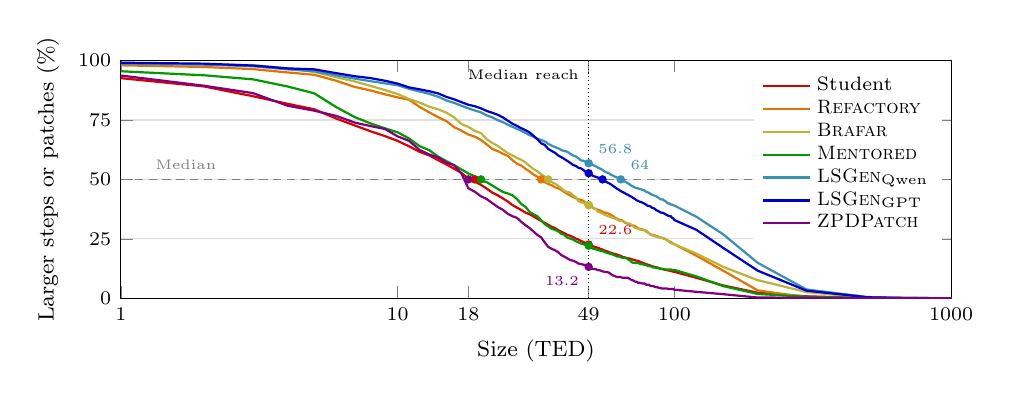
\begin{tikzpicture}
\begin{axis}[width=\columnwidth, height=4.6cm, xmode=log, xmin=1, xmax=1000, ymin=0, ymax=100,
 xtick={1,10,18,49,100,1000}, xticklabels={1,10,18,49,100,1000}, ytick={0,25,50,75,100},
 xlabel={Size (TED)}, ylabel={Larger steps or patches (\%)}, ymajorgrids, grid style={gray!25},
 legend cell align=left, legend style={at={(0.99,0.98)}, anchor=north east, fill=white, row sep=-2pt}]
% rows:patchsize
\addplot[referenceline] coordinates {(1,92.6) (2,89.1) (3,85.0) (4,81.8) (5,79.5) (6,75.6) (7,72.7) (8,70.2) (9,68.2) (10,66.2) (11,63.9) (12,61.6) (13,60.1) (14,58.1) (15,56.3) (16,54.5) (17,52.7) (18,50.4) (19,49.1) (20,47.7) (21,46.1) (22,44.4) (23,43.3) (24,42.0) (25,40.7) (26,39.2) (27,38.1) (28,37.1) (29,36.0) (30,35.3) (31,34.4) (32,33.4) (33,32.6) (34,31.7) (35,30.9) (36,30.1) (37,29.5) (38,28.7) (39,28.0) (40,27.4) (41,26.7) (42,26.3) (43,25.7) (44,25.1) (45,24.7) (46,24.1) (47,23.6) (48,23.0) (49,22.6) (50,22.2) (51,21.8) (52,21.5) (53,21.2) (54,20.8) (55,20.5) (56,20.0) (57,19.8) (58,19.4) (59,19.1) (60,18.8) (61,18.6) (62,18.4) (63,18.1) (64,17.8) (65,17.4) (66,17.2) (67,17.0) (68,16.8) (69,16.7) (70,16.4) (71,16.2) (72,16.0) (73,15.8) (74,15.7) (75,15.4) (76,15.1) (77,14.9) (78,14.6) (79,14.4) (80,14.1) (81,14.0) (82,13.7) (83,13.5) (84,13.3) (85,13.2) (86,13.0) (87,12.9) (88,12.7) (89,12.5) (90,12.4) (91,12.2) (92,12.0) (93,11.9) (94,11.8) (95,11.7) (96,11.6) (97,11.5) (98,11.3) (99,11.2) (100,11.1) (120,8.6) (150,5.4) (200,2.3) (300,0.8) (500,0.1) (700,0.0) (1000,0.0)};
\addplot[refactoryline] coordinates {(1,98.0) (2,97.3) (3,96.4) (4,95.0) (5,94.0) (6,91.5) (7,88.9) (8,87.4) (9,85.8) (10,84.5) (11,83.5) (12,80.5) (13,78.2) (14,76.2) (15,74.5) (16,72.0) (17,70.5) (18,68.9) (19,68.0) (20,66.6) (21,64.7) (22,62.8) (23,61.9) (24,60.8) (25,59.9) (26,58.1) (27,56.6) (28,55.8) (29,54.4) (30,53.3) (31,52.0) (32,51.1) (33,49.6) (34,48.8) (35,48.1) (36,47.6) (37,46.7) (38,46.3) (39,45.6) (40,44.7) (41,43.9) (42,43.3) (43,42.6) (44,42.1) (45,41.6) (46,41.4) (47,40.9) (48,40.0) (49,39.2) (50,38.7) (51,37.8) (52,37.6) (53,37.2) (54,36.9) (55,36.4) (56,36.0) (57,35.9) (58,35.5) (59,35.0) (60,34.6) (61,33.9) (62,33.5) (63,33.1) (64,32.9) (65,32.7) (66,31.9) (67,31.6) (68,31.3) (69,31.2) (70,30.7) (71,30.6) (72,30.3) (73,29.9) (74,29.4) (75,29.2) (76,29.0) (77,28.9) (78,28.7) (79,28.4) (80,27.7) (81,27.3) (82,26.9) (83,26.7) (84,26.6) (85,26.4) (86,26.1) (87,26.1) (88,25.7) (89,25.6) (90,25.3) (91,25.2) (92,25.0) (93,24.8) (94,24.5) (95,24.2) (96,23.8) (97,23.7) (98,23.3) (99,22.9) (100,22.7) (120,17.9) (150,11.6) (200,3.3) (300,0.4) (500,0.0) (700,0.0) (1000,0.0)};
\addplot[brafarline] coordinates {(1,99.0) (2,98.4) (3,98.1) (4,96.7) (5,95.2) (6,93.0) (7,91.2) (8,89.3) (9,87.6) (10,85.9) (11,83.8) (12,82.3) (13,80.6) (14,79.5) (15,78.1) (16,76.1) (17,73.3) (18,72.1) (19,70.4) (20,69.5) (21,66.9) (22,65.3) (23,64.1) (24,62.5) (25,61.1) (26,60.1) (27,59.0) (28,58.2) (29,57.1) (30,55.6) (31,54.3) (32,53.4) (33,52.2) (34,51.2) (35,49.9) (36,48.9) (37,48.2) (38,47.3) (39,46.3) (40,45.2) (41,44.7) (42,44.4) (43,43.3) (44,42.6) (45,40.9) (46,40.3) (47,40.1) (48,39.7) (49,39.2) (50,38.7) (51,38.0) (52,37.5) (53,36.4) (54,36.1) (55,35.6) (56,35.1) (57,34.7) (58,34.4) (59,34.1) (60,33.8) (61,33.5) (62,33.2) (63,32.7) (64,32.5) (65,32.4) (66,32.1) (67,31.8) (68,31.4) (69,31.3) (70,30.8) (71,30.2) (72,29.6) (73,29.4) (74,29.3) (75,28.9) (76,28.8) (77,28.7) (78,28.5) (79,28.0) (80,27.9) (81,27.4) (82,26.7) (83,26.5) (84,26.3) (85,26.1) (86,25.9) (87,25.8) (88,25.7) (89,25.6) (90,25.5) (91,25.4) (92,25.2) (93,24.9) (94,24.5) (95,24.0) (96,23.6) (97,23.2) (98,23.0) (99,22.9) (100,22.7) (120,18.8) (150,13.2) (200,7.6) (300,2.6) (500,0.2) (700,0.2) (1000,0.0)};
\addplot[mentoredline] coordinates {(1,95.5) (2,93.8) (3,92.1) (4,89.1) (5,86.2) (6,80.4) (7,76.2) (8,73.5) (9,71.5) (10,69.8) (11,67.2) (12,64.0) (13,62.3) (14,59.6) (15,57.7) (16,56.0) (17,54.2) (18,52.5) (19,51.3) (20,49.6) (21,48.8) (22,47.4) (23,46.0) (24,44.7) (25,44.1) (26,43.3) (27,41.7) (28,39.6) (29,38.4) (30,36.3) (31,35.3) (32,34.5) (33,32.8) (34,31.2) (35,30.2) (36,29.2) (37,28.8) (38,28.2) (39,27.1) (40,26.7) (41,25.5) (42,25.1) (43,24.7) (44,24.0) (45,23.5) (46,23.0) (47,22.7) (48,22.4) (49,22.1) (50,21.4) (51,20.7) (52,20.6) (53,20.3) (54,20.0) (55,19.9) (56,19.4) (57,19.1) (58,18.9) (59,18.6) (60,18.3) (61,18.0) (62,17.6) (63,17.6) (64,17.2) (65,17.0) (66,16.9) (67,16.9) (68,16.3) (69,16.0) (70,15.2) (71,14.9) (72,14.9) (73,14.8) (74,14.8) (75,14.5) (76,14.3) (77,14.3) (78,14.0) (79,14.0) (80,13.6) (81,13.6) (82,13.3) (83,13.3) (84,12.9) (85,12.9) (86,12.8) (87,12.8) (88,12.5) (89,12.3) (90,12.3) (91,12.3) (92,12.2) (93,12.1) (94,12.1) (95,12.1) (96,12.1) (97,12.1) (98,11.9) (99,11.9) (100,11.9) (120,9.2) (150,5.1) (200,1.8) (300,0.6) (500,0.1) (700,0.0) (1000,0.0)};
\addplot[qwenline] coordinates {(1,98.7) (2,98.3) (3,97.6) (4,96.3) (5,95.5) (6,93.8) (7,92.4) (8,91.3) (9,90.4) (10,89.6) (11,88.1) (12,87.0) (13,86.0) (14,84.8) (15,83.2) (16,82.2) (17,81.0) (18,79.9) (19,79.0) (20,78.2) (21,76.9) (22,76.1) (23,74.9) (24,74.1) (25,73.0) (26,72.1) (27,71.3) (28,70.4) (29,69.5) (30,68.6) (31,67.9) (32,67.1) (33,66.6) (34,66.0) (35,65.0) (36,64.2) (37,63.6) (38,63.1) (39,62.4) (40,61.9) (41,61.7) (42,60.8) (43,60.1) (44,59.7) (45,58.9) (46,58.0) (47,57.8) (48,57.3) (49,56.8) (50,56.6) (51,56.0) (52,55.5) (53,54.9) (54,54.5) (55,54.0) (56,53.3) (57,52.9) (58,52.6) (59,51.9) (60,51.6) (61,51.1) (62,50.8) (63,50.4) (64,49.9) (65,49.4) (66,49.2) (67,48.8) (68,48.3) (69,47.9) (70,47.3) (71,47.0) (72,46.6) (73,46.3) (74,46.2) (75,45.9) (76,45.8) (77,45.5) (78,45.3) (79,44.8) (80,44.6) (81,44.3) (82,43.9) (83,43.5) (84,43.4) (85,43.1) (86,42.9) (87,42.5) (88,42.1) (89,41.7) (90,41.5) (91,41.5) (92,41.0) (93,40.8) (94,40.2) (95,39.9) (96,39.9) (97,39.4) (98,39.4) (99,39.1) (100,39.0) (120,34.3) (150,26.9) (200,14.9) (300,3.7) (500,0.5) (700,0.1) (1000,0.0)};
\addplot[gptline] coordinates {(1,99.1) (2,98.7) (3,97.9) (4,96.7) (5,96.3) (6,94.7) (7,93.4) (8,92.6) (9,91.5) (10,90.3) (11,88.7) (12,87.9) (13,87.1) (14,86.2) (15,84.7) (16,83.7) (17,82.5) (18,81.4) (19,80.8) (20,79.9) (21,78.8) (22,78.0) (23,77.2) (24,76.1) (25,74.7) (26,73.4) (27,72.5) (28,71.5) (29,70.7) (30,69.7) (31,68.3) (32,66.9) (33,65.2) (34,64.5) (35,62.8) (36,62.0) (37,61.2) (38,60.1) (39,59.4) (40,58.6) (41,57.8) (42,57.0) (43,56.1) (44,55.7) (45,54.9) (46,54.6) (47,53.9) (48,52.9) (49,52.6) (50,52.0) (51,51.4) (52,51.1) (53,50.7) (54,50.5) (55,50.0) (56,49.3) (57,48.8) (58,48.4) (59,47.9) (60,47.3) (61,46.7) (62,46.1) (63,45.6) (64,45.1) (65,44.7) (66,44.3) (67,43.8) (68,43.5) (69,43.0) (70,42.7) (71,42.2) (72,41.8) (73,41.2) (74,40.9) (75,40.6) (76,40.4) (77,40.1) (78,39.8) (79,39.4) (80,38.9) (81,38.8) (82,38.6) (83,38.1) (84,37.9) (85,37.6) (86,37.0) (87,36.8) (88,36.5) (89,36.1) (90,36.0) (91,35.9) (92,35.6) (93,35.3) (94,35.0) (95,34.7) (96,34.6) (97,34.5) (98,33.9) (99,33.6) (100,32.9) (120,28.8) (150,21.2) (200,11.6) (300,3.2) (500,0.4) (700,0.1) (1000,0.0)};
\addplot[proposedline] coordinates {(1,93.7) (2,89.4) (3,86.3) (4,81.0) (5,78.9) (6,76.7) (7,73.9) (8,72.4) (9,71.2) (10,68.1) (11,66.2) (12,62.4) (13,60.5) (14,59.2) (15,57.1) (16,55.9) (17,52.5) (18,46.3) (19,44.8) (20,42.9) (21,41.7) (22,40.0) (23,38.4) (24,37.2) (25,35.5) (26,34.5) (27,33.8) (28,32.1) (29,30.7) (30,29.5) (31,28.0) (32,26.6) (33,25.6) (34,23.5) (35,21.6) (36,20.8) (37,20.2) (38,19.4) (39,18.2) (40,17.5) (41,16.8) (42,16.1) (43,15.8) (44,15.3) (45,14.6) (46,14.4) (47,14.1) (48,13.9) (49,13.2) (50,12.5) (51,12.3) (52,12.2) (53,11.8) (54,11.7) (55,11.3) (56,11.1) (57,11.0) (58,10.8) (59,10.1) (60,9.6) (61,9.3) (62,8.9) (63,8.9) (64,8.9) (65,8.6) (66,8.6) (67,8.6) (68,8.6) (69,8.1) (70,7.7) (71,7.5) (72,7.0) (73,6.9) (74,6.5) (75,6.5) (76,6.3) (77,6.2) (78,6.2) (79,5.7) (80,5.7) (81,5.7) (82,5.1) (83,5.1) (84,5.1) (85,4.8) (86,4.6) (87,4.6) (88,4.3) (89,4.3) (90,4.1) (91,4.1) (92,4.1) (93,4.1) (94,4.1) (95,3.9) (96,3.9) (97,3.9) (98,3.9) (99,3.8) (100,3.6) (120,2.7) (150,1.7) (200,0.3) (300,0.2) (500,0.0) (700,0.0) (1000,0.0)};
\addplot[referenceline, forget plot, only marks, mark=*, mark size=1.1pt] coordinates {(49,22.6) (19,50)};
\addplot[refactoryline, forget plot, only marks, mark=*, mark size=1.1pt] coordinates {(49,39.2) (33,50)};
\addplot[brafarline, forget plot, only marks, mark=*, mark size=1.1pt] coordinates {(49,39.2) (35,50)};
\addplot[mentoredline, forget plot, only marks, mark=*, mark size=1.1pt] coordinates {(49,22.1) (20,50)};
\addplot[qwenline, forget plot, only marks, mark=*, mark size=1.1pt] coordinates {(49,56.8) (64,50)};
\addplot[gptline, forget plot, only marks, mark=*, mark size=1.1pt] coordinates {(49,52.6) (55,50)};
\addplot[proposedline, forget plot, only marks, mark=*, mark size=1.1pt] coordinates {(49,13.2) (18,50)};
% end rows
\draw[densely dotted] (axis cs:49,0) -- (axis cs:49,100) node[pos=0.94, anchor=east, font=\tiny] {Median reach};
\node[font=\tiny, violet, anchor=north east] at (axis cs:49,13.2) {13.2};
\node[font=\tiny, red!85!black, anchor=south west] at (axis cs:49,22.6) {22.6};
\node[font=\tiny, cyan!70!black, anchor=south west] at (axis cs:49,56.8) {56.8};
\node[font=\tiny, cyan!70!black, anchor=south west] at (axis cs:64,50) {64};
\draw[densely dashed, gray] (axis cs:1,50) -- (axis cs:1000,50) node[pos=0.03, anchor=south west, font=\tiny] {Median};
\legend{Student, \textsc{Refactory}, \textsc{Brafar}, \textsc{Mentored}, \textsc{LSGen}\textsubscript{Qwen}, \textsc{LSGen}\textsubscript{GPT}, \textsc{ZPDPatch}}
\end{axis}
\end{tikzpicture}%
\caption{Size distributions of students' steps and of each technique's patches}
\label{fig:patchsize}
\end{figure}

% Figure~\ref{fig:patchsize}는 각 크기보다 큰 학생 걸음과 각 기법 patch의 비율을 그린다. \textsc{ZPDPatch}의 곡선은 모든 크기에서 기존 기법의 곡선 아래에 놓였고, 중앙값인 TED 18부터는 학생 걸음의 곡선보다도 아래에 놓였다. 기존 기법 가운데 학생 걸음의 곡선에 가장 가까운 \textsc{Mentored}도 모든 크기에서 \textsc{ZPDPatch}의 곡선 위에 있었다. demonstrated reach의 중앙값인 TED 49를 넘는 것은 \textsc{ZPDPatch}의 patch 가운데 13.2\%뿐이었고, 학생 걸음은 22.6\%, 기존 기법의 patch는 22.1--56.8\%였다. 따라서 어느 크기를 기준으로 하든 그보다 큰 patch를 가장 작은 비율로 돌려준 것은 \textsc{ZPDPatch}였다.
Figure~\ref{fig:patchsize} plots the share of the students' steps and of each technique's patches that are larger than each size. The curve of \textsc{ZPDPatch} lay below those of the existing techniques at every size and, from its median TED of 18 on, below that of the student steps as well. \textsc{Mentored}, the existing technique whose curve was closest to that of the student steps, also lay above \textsc{ZPDPatch} at every size. Only 13.2\% of the patches of \textsc{ZPDPatch} exceeded a TED of 49, the median demonstrated reach, against 22.6\% of the student steps and 22.1--56.8\% of the patches of the existing techniques. Hence, whatever size is taken, \textsc{ZPDPatch} returned the smallest share of patches larger than that size.

\begin{table}[h]
\caption{Repairs of each technique against the students' own steps and fixes}
\label{tab:rq1}
\centering\footnotesize
\setlength{\tabcolsep}{3pt}
\begin{tabular}{@{}l||rr|rr|rrr@{}}
\toprule
 & \multicolumn{2}{c|}{Within reach} & \multicolumn{2}{c|}{Retention (\%)} & \multicolumn{3}{c}{Student's fix (\%)} \\
 & Fixed & Problems & & & No & Within & Same \\
 & (\%) & ($\geq$70\%) & Tokens & Lines & larger & TED 10 & AST \\
\midrule
% rows:rq1
Students & -- & -- & 96.4 & 85.7 & -- & -- & -- \\
\midrule
\textsc{Refactory} & 56.5 & 4/12 & 71.3 & 22.2 & 34.0 & 13.0 & 3.2 \\
\textsc{Brafar} & 58.3 & 3/14 & 65.7 & 20.0 & 31.6 & 10.8 & 1.9 \\
\textsc{Mentored} & 70.9 & 7/14 & 84.2 & 40.0 & 46.5 & 23.1 & 7.7 \\
\textsc{LSGen}\textsubscript{Qwen} & 42.2 & 1/14 & 62.3 & 25.0 & 23.0 & 10.1 & 3.8 \\
\textsc{LSGen}\textsubscript{GPT} & 46.3 & 0/14 & 65.2 & 25.0 & 26.3 & 10.4 & 4.4 \\
\midrule
\textsc{ZPDPatch} & 76.7 & 11/14 & 96.2 & 83.3 & 56.6 & 32.9 & 16.3 \\
% end rows
\bottomrule
\end{tabular}
\end{table}

% Table~\ref{tab:rq1}은 모든 기법의 수리를 학생 자신의 걸음 및 수정과 비교한다. \textsc{ZPDPatch}가 수리한 프로그램 가운데 76.7\%가 학생의 demonstrated reach 안에 들었고, 기존 기법은 42.2--70.9\%였다. 이 비율이 70\%에 이르는 문제는 14개 가운데 11개로, 어느 기존 기법이든 많아야 7개였다. Retention은 patch가 버기 프로그램의 token과 줄을 중앙값으로 얼마나 남기는지 보인다. \textsc{ZPDPatch}의 patch는 학생의 코드를 학생 걸음과 거의 같게 남겨, 버기 프로그램 token의 96.2\%와 줄의 83.3\%를 남겼고, 학생 걸음은 96.4\%와 85.7\%, 기존 기법은 많아야 84.2\%와 40.0\%였다. 이는 \textsc{ZPDPatch}의 target이 학생 자신의 이후 제출인 반면, 기존 기법은 test suite를 통과하는 어떤 프로그램이든 향하기 때문이다(RQ3). Student's fix는 patch를 학생 자신의 accepted 프로그램과 비교한다. \textsc{ZPDPatch}의 patch 가운데 56.6\%는 accepted까지 내디딘 학생 자신의 걸음보다 크지 않았고, 32.9\%는 accepted 프로그램에서 TED 10 이내였으며, 16.3\%는 학습도 수리도 그 프로그램을 보지 않았는데도 그 프로그램과 AST가 정확히 같았다. 기존 기법은 많아야 각각 46.5\%, 23.1\%, 7.7\%였다. 따라서 \textsc{ZPDPatch}의 수리는 기존 기법의 수리보다 더 자주 학생의 reach 안에 들었고, 학생의 코드를 학생 걸음과 거의 같게 남겼으며, 학생 자신의 accepted 프로그램에 더 가까웠다.
Table~\ref{tab:rq1} compares the repairs of every technique with the students' own steps and fixes. Of the fixed programs of \textsc{ZPDPatch}, 76.7\% lay within the student's demonstrated reach, against 42.2--70.9\% for the existing techniques. The share reached 70\% on 11 of the 14 problems, against at most 7 for any existing technique. Retention shows the median share of the buggy program's tokens and lines that a patch keeps. A patch of \textsc{ZPDPatch} kept nearly as much of the student's code as a student step does, 96.2\% of the buggy program's tokens and 83.3\% of its lines, against 96.4\% and 85.7\% for a student step and at most 84.2\% and 40.0\% for the existing techniques. This is because the targets of \textsc{ZPDPatch} are the student's own later submissions, whereas the existing techniques head for any program that passes the test suite (RQ3). Student's fix compares a patch with the student's own accepted program. Of the patches of \textsc{ZPDPatch}, 56.6\% were no larger than the student's own step to acceptance, 32.9\% were within a TED of 10 of the accepted program, and 16.3\% had exactly its AST although neither training nor repair saw that program. The existing techniques reached at most 46.5\%, 23.1\%, and 7.7\%, respectively. Hence, the repairs of \textsc{ZPDPatch} lay within the student's reach more often than those of the existing techniques, kept nearly as much of the student's code as a student step does, and came closer to the student's own accepted program.

\begin{table}[h]
\caption{Forward steps of students and of \textsc{ZPDPatch}}
\label{tab:rq1steps}
\centering\footnotesize
\begin{tabular}{@{}l||rr@{}}
\toprule
 & Students & \textsc{ZPDPatch} \\
\midrule
% rows:rq1steps
Forward steps & 1,397 & 111 \\
\midrule
WA $\to$ WA (\%) & 93.5 & 91.0 \\
TLE $\to$ WA (\%) & 4.5 & 5.4 \\
Other (\%) & 2.0 & 3.6 \\
\midrule
Pass rate gain (points) & 12.5 & 12.5 \\
Pass rate gain (\%) & 17.6 & 18.2 \\
TED & 17 & 14 \\
% end rows
\bottomrule
\end{tabular}
\end{table}

% Table~\ref{tab:rq1steps}는 \textsc{ZPDPatch}가 수리하지 못한 버기 프로그램에서 돌려준 앞으로 나아간 걸음(Algorithm~\ref{alg:construct}의 21--23번째 줄) 111개를 학생의 앞으로 나아간 걸음 1,397개와 비교한다. 둘은 verdict 변화의 구성이 비슷하여, 학생 걸음의 93.5\%와 \textsc{ZPDPatch} 걸음의 91.0\%가 WA verdict를 유지한 채 더 많은 test case를 통과했고, 각각 4.5\%와 5.4\%가 Time Limit Exceeded(TLE)에서 WA로 옮겨 갔다. 걸음당 pass rate 이득의 중앙값은 둘 다 12.5 포인트였고, 걸음의 크기도 TED 17과 14로 비슷했다. 따라서 \textsc{ZPDPatch}가 수리하지 못한 버기 프로그램에서 돌려준 앞으로 나아간 걸음은 verdict 변화, pass rate 이득, 크기 모두에서 학생 자신의 앞으로 나아간 걸음과 비슷했다.
Table~\ref{tab:rq1steps} compares the 111 forward steps that \textsc{ZPDPatch} returned on the buggy programs it did not repair (lines~21--23 of Algorithm~\ref{alg:construct}) with the 1,397 forward steps of the students. The two had a similar mix of verdict changes: 93.5\% of the student steps and 91.0\% of those of \textsc{ZPDPatch} passed more test cases while keeping the WA verdict, and 4.5\% and 5.4\% moved from Time Limit Exceeded (TLE) to WA. The median pass-rate gain per step was 12.5 points for both, and the steps were of similar size, with a TED of 17 and 14. Hence, the forward steps that \textsc{ZPDPatch} returned on the buggy programs it did not repair were similar to the students' own forward steps in verdict change, pass-rate gain, and size.

% 이 결과들은 \textsc{ZPDPatch}의 patch가 기존 기법의 patch보다 작고 더 큰 비율이 reach 안에 머물며 학생의 코드를 학생 걸음과 거의 같게 남긴다는 것, 그리고 \textsc{ZPDPatch}가 수리하지 못하는 버기 프로그램에서 돌려주는 앞으로 나아간 걸음이 학생 자신의 앞으로 나아간 걸음을 닮았다는 것을 보여 준다.
These results show that the patches of \textsc{ZPDPatch} are smaller than those of the existing techniques, stay within reach more often, and keep nearly as much of the student's code as a student step does, and that the forward steps it returns on the buggy programs it does not repair resemble the students' own forward steps.

\subsection{RQ2: Replacing and Complementing Existing Techniques}
\label{sec:rq-comparison}

% RQ2에 답하기 위해, 우리는 RQ1 벤치마크의 버기 프로그램 1,753개에서 \textsc{ZPDPatch}를 각 기존 구성 대신 쓸 때와 그 앞에 둘 때를 그 구성 단독과 비교했다.
To answer RQ2, we compared \textsc{ZPDPatch}, used instead of and before each existing configuration, with that configuration alone on the 1,753 buggy programs of the RQ1 benchmark.

\begin{table}[h]
\caption{\textsc{ZPDPatch} against each existing technique}
\label{tab:rq2}
\centering\footnotesize
\begin{tabular}{@{}l||rr|rrr@{}}
\toprule
 & \multicolumn{2}{c|}{} & \multicolumn{3}{c}{\textsc{ZPDPatch} where} \\
 & \multicolumn{2}{c|}{All (\%)} & \multicolumn{3}{c}{both repair (\%)} \\
 & & Beyond & Smaller & More & More \\
 & RR & reach & TED & tokens & lines \\
\midrule
% rows:rq2
\textsc{Refactory} & 54.3 & 23.6 & 45.0 & 19.2 & 155.9 \\
\textsc{Brafar} & 54.9 & 22.9 & 49.1 & 27.4 & 149.1 \\
\textsc{Mentored} & 40.2 & 11.7 & 13.4 & 7.0 & 72.0 \\
\textsc{LSGen}\textsubscript{Qwen} & 79.4 & 45.9 & 60.9 & 27.6 & 102.7 \\
\textsc{LSGen}\textsubscript{GPT} & 92.1 & 49.5 & 51.9 & 24.5 & 102.3 \\
\midrule
\textsc{ZPDPatch} & 33.3 & 7.8 & -- & -- & -- \\
% end rows
\bottomrule
\end{tabular}
\end{table}

% Table~\ref{tab:rq2}는 모든 버기 프로그램에서 각 기법의 수리를, 그리고 \textsc{ZPDPatch}와 각 기존 구성이 모두 수리한 버기 프로그램에서 둘의 patch를 비교한다. \textsc{ZPDPatch}는 기존 구성보다 버기 프로그램을 17.3--63.9\% 더 적게 수리했다. 이는 \textsc{ZPDPatch}의 목표에서 오는 예상된 결과다. 기존 기법은 test suite를 통과하는 어떤 프로그램이든 향하는 반면, \textsc{ZPDPatch}는 학생의 ZPD 안의 걸음을 향하므로, 학생 자신도 큰 걸음을 내디뎌야 했던 버기 프로그램을 수리하지 못하고 남겼다. 실제로 \textsc{ZPDPatch}가 수리하지 못한 버기 프로그램에서는 accepted 프로그램까지 내디딘 학생 자신의 걸음이 수리한 버기 프로그램에서보다 평균 68.9\% 더 컸다. RR은 낮았지만, RQ1에서 보았듯이 \textsc{ZPDPatch}가 목표로 한 것, 즉 수리가 학생의 reach 안에 드는 비율은 76.7\%로 기존 기법(42.2--70.9\%)보다 높았다(Table~\ref{tab:rq1}). 같은 이유로, \textsc{ZPDPatch}는 학생의 reach 밖인 plausible patch를 모든 버기 프로그램의 7.8\%에서만 돌려주어, 기존 구성(11.7--49.5\%)보다 33.7--84.3\% 더 적었다. 수리하지 못한 버기 프로그램에서 기존 기법은 구현된 대로 제출 자체를 돌려준 반면, \textsc{ZPDPatch}는 그 가운데 9.5\%에서 앞으로 나아간 걸음(Table~\ref{tab:rq1steps})을 돌려주었고, 그 85.6\%가 학생의 reach 안에 있었다. 둘이 모두 수리한 버기 프로그램에서, \textsc{ZPDPatch}의 patch는 다섯 구성 각각의 patch보다 TED가 13.4--60.9\% 작았고, 학생의 token을 7.0--27.6\%, 줄을 72.0--155.9\% 더 많이 남겼다. 따라서 기존 기법 대신 \textsc{ZPDPatch}를 쓰면 수리는 줄지만, reach 밖의 patch가 줄고, 수리하지 못한 버기 프로그램 일부에서는 앞으로 나아간 걸음을 받으며, 같은 버기 프로그램에서는 더 작고 학생의 코드를 더 많이 남기는 patch를 받는다.
Table~\ref{tab:rq2} compares the repairs of each technique on all buggy programs, and the patches of \textsc{ZPDPatch} and of each existing configuration on the buggy programs both repair. \textsc{ZPDPatch} repaired 17.3--63.9\% fewer buggy programs than the existing configurations. This is an expected consequence of its goal. Whereas the existing techniques head for any program that passes the test suite, \textsc{ZPDPatch} heads for a step within the student's ZPD, so it left unrepaired the buggy programs on which the students themselves had to take large steps. Indeed, on the buggy programs \textsc{ZPDPatch} did not repair, the students' own steps to their accepted programs were 68.9\% larger on average than on those it repaired. Although its RR was lower, the share of its repairs within the student's reach, which \textsc{ZPDPatch} aims at, was 76.7\% as RQ1 showed, higher than the 42.2--70.9\% of the existing techniques (Table~\ref{tab:rq1}). For the same reason, \textsc{ZPDPatch} returned a plausible patch beyond the student's reach on only 7.8\% of all buggy programs, 33.7--84.3\% fewer than the existing configurations (11.7--49.5\%). On the buggy programs they did not repair, the existing techniques, as implemented, returned the submission itself, whereas \textsc{ZPDPatch} returned a forward step (Table~\ref{tab:rq1steps}) on 9.5\% of them, 85.6\% of which lay within the student's reach. On the buggy programs both repair, the patches of \textsc{ZPDPatch} had a 13.4--60.9\% smaller TED than those of each of the five configurations and kept 7.0--27.6\% more of the student's tokens and 72.0--155.9\% more of the lines. Hence, using \textsc{ZPDPatch} instead of an existing technique repairs fewer buggy programs, but returns fewer patches beyond reach, gives a forward step on some of the buggy programs it does not repair, and on the same buggy programs gives smaller patches that keep more of the student's code.

\begin{figure}[h]
\centering
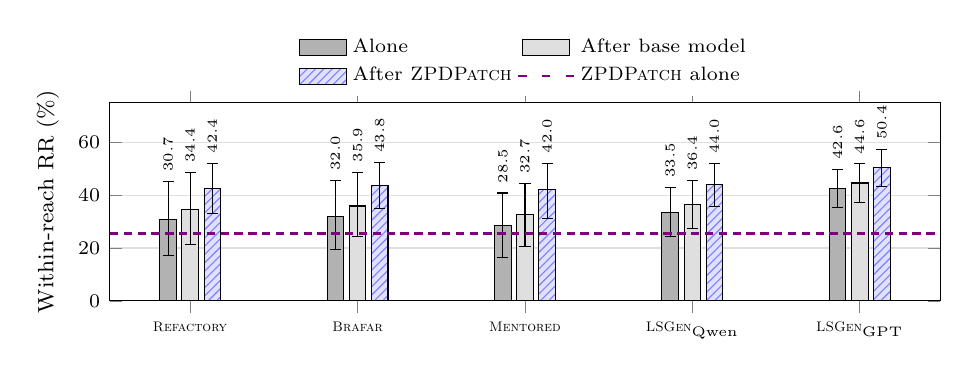
\begin{tikzpicture}
\begin{axis}[ybar, disabledatascaling, width=\columnwidth, height=4.1cm, bar width=6pt, enlarge x limits=0.12,
 symbolic x coords={refactory,brafar,mentored,lsgen_qwen,lsgen}, xtick=data, xticklabels={\textsc{Refactory}, \textsc{Brafar}, \textsc{Mentored}, \textsc{LSGen}\textsubscript{Qwen}, \textsc{LSGen}\textsubscript{GPT}}, x tick label style={font=\tiny},
 ymin=0, ymax=75, ytick={0,20,40,60}, ylabel={Within-reach RR (\%)}, ymajorgrids, grid style={gray!25},
 nodes near coords={\pgfmathprintnumber[fixed, fixed zerofill, precision=1]{\pgfplotspointmeta}}, visualization depends on={\thisrow{p} \as \ep}, every node near coord/.append style={font=\tiny, yshift=\ep*\pgfplotsunitylength, rotate=90, anchor=west},
 legend columns=2, area legend, legend cell align=left, legend style={at={(0.5,1.03)}, anchor=south}]
% rows:combined
\addplot[baseline2, error bars/.cd, y dir=both, y explicit] table[row sep=\\, y=v, x=at, y error plus=p, y error minus=m] {v at p m\\ 30.7 refactory 14.5 13.7\\ 32.0 brafar 13.5 12.4\\ 28.5 mentored 12.3 12.2\\ 33.5 lsgen_qwen 9.4 9.2\\ 42.6 lsgen 7.1 7.3\\};
\addplot[variant, error bars/.cd, y dir=both, y explicit] table[row sep=\\, y=v, x=at, y error plus=p, y error minus=m] {v at p m\\ 34.4 refactory 14.2 13.2\\ 35.9 brafar 12.8 11.4\\ 32.7 mentored 11.8 12.0\\ 36.4 lsgen_qwen 9.2 9.0\\ 44.6 lsgen 7.2 7.5\\};
\addplot[proposed, error bars/.cd, y dir=both, y explicit] table[row sep=\\, y=v, x=at, y error plus=p, y error minus=m] {v at p m\\ 42.4 refactory 9.7 9.5\\ 43.8 brafar 8.6 8.7\\ 42.0 mentored 10.1 10.8\\ 44.0 lsgen_qwen 8.0 8.4\\ 50.4 lsgen 6.8 7.3\\};
\draw[violet, densely dashed, thick] ({rel axis cs:0,0} |- {axis cs:refactory,25.5}) -- ({rel axis cs:1,0} |- {axis cs:refactory,25.5});
% end rows
\addlegendimage{line legend, violet, densely dashed, thick}
\legend{Alone, After base model, After \textsc{ZPDPatch}, \textsc{ZPDPatch} alone}
\end{axis}
\end{tikzpicture}
\caption{Within-reach repair rate of each existing technique alone, after the base model, and after \textsc{ZPDPatch}}
\label{fig:combined}
\end{figure}

% 정답 프로그램이 필요할 때는, \textsc{ZPDPatch}가 수리하지 못한 버기 프로그램을 그 뒤에 둔 기존 기법이 수리할 수 있다. Figure~\ref{fig:combined}은 각 기존 기법을 단독으로 쓸 때, 같은 수의 후보를 내는 학습하지 않은 base model 뒤에 둘 때, \textsc{ZPDPatch} 뒤에 둘 때의 reach 안 수리율을 그린다. 단독으로 쓴 \textsc{ZPDPatch}의 reach 안 수리율 25.5\%(점선)는 기존 기법 단독의 28.5--42.6\%보다 낮았다. 그러나 \textsc{ZPDPatch} 뒤에 두면 각 기법의 reach 안 수리율이 18.3--47.4\%, 즉 7.8--13.5 포인트 올랐고, 문제에 걸친 그 이득의 95\% bootstrap 구간은 4.3 포인트보다 위에 있었으며, 14개 문제 가운데 11--13개에서 올랐다. base model 뒤에 두면 4.7--14.8\%만 올라, 이 이득은 후보를 더한 것만으로는 설명되지 않았다. \textsc{ZPDPatch} 뒤에 두면 RR도 1.1--42.3\% 올랐다. 따라서 \textsc{ZPDPatch}를 기존 기법 앞에 두면 그 기법의 RR과 reach 안 수리율이 모두 올랐다.
When a correct program is required, an existing technique placed after \textsc{ZPDPatch} can repair the buggy programs that \textsc{ZPDPatch} does not repair. Figure~\ref{fig:combined} plots the within-reach repair rate of each existing technique alone, placed after the untrained base model drawing the same number of candidates, and placed after \textsc{ZPDPatch}. The within-reach repair rate of \textsc{ZPDPatch} alone, 25.5\% (dashed line), was below the 28.5--42.6\% of the existing techniques alone. Placed after \textsc{ZPDPatch}, however, each technique's within-reach repair rate rose by 18.3--47.4\%, or 7.8--13.5 points, with 95\% bootstrap intervals of the gain over problems above 4.3 points, and it rose on 11--13 of the 14 problems. Placed after the base model, it rose by only 4.7--14.8\%, so extra candidates alone did not explain the gain. After \textsc{ZPDPatch}, the RR also rose by 1.1--42.3\%. Hence, placing \textsc{ZPDPatch} before an existing technique raised both that technique's RR and its within-reach repair rate.

% 이 결과들은 \textsc{ZPDPatch}가 단독으로는 기존 기법보다 버기 프로그램을 더 적게 수리하지만, reach 밖의 patch를 더 적게 돌려주고 같은 버기 프로그램에서는 더 작은 patch를 돌려주며, 기존 기법 앞에 두면 그 기법의 RR과 reach 안 수리율을 모두 높인다는 것을 보여 준다.
These results show that \textsc{ZPDPatch} alone repairs fewer buggy programs than the existing techniques, but returns fewer patches beyond reach and smaller patches on the same buggy programs, and that placed before an existing technique, it raises both that technique's RR and its within-reach repair rate.

\subsection{RQ3: Ablation Study}
\label{sec:rq-ablation}

% RQ3에 답하기 위해, 우리는 \textsc{ZPDPatch}의 설계 선택 네 가지를 하나씩 바꾼 변형을 Seen과 Unseen에서 비교했다. \textsc{ZPDPatch}-Train은 학습(Algorithm~\ref{alg:construct}의 10--11번째 줄)을 제거하고 base model로 생성한다. \textsc{ZPDPatch}-Cascade는 cascade를 checkpoint 하나로 줄인다. \textsc{ZPDPatch}-Distinct는 서로 다른 세 checkpoint 대신 한 checkpoint에서 후보 세 개를 뽑는다. \textsc{ZPDPatch}+History는 학생의 이전 제출을 prompt에 덧붙인다. Figure~\ref{fig:ablation}은 Seen과 Unseen에서 각 변형이 그 선택을 갖춘 구성보다 버기 프로그램을 몇 \% 더 적게 수리하는지 그린다. \(\dagger\)로 표시한 선택은 양쪽 모두 현재 제출만 담은 prompt로 temperature 0.8에서 후보 세 개를 뽑아, 학습은 base model과 checkpoint 하나를, 서로 다른 checkpoint는 checkpoint 하나와 세 개를 비교한다.
To answer RQ3, we compared variants that each change one of four design choices of \textsc{ZPDPatch} on Seen and Unseen. \textsc{ZPDPatch}-Train removes training (lines~10--11 of Algorithm~\ref{alg:construct}) and generates with the base model. \textsc{ZPDPatch}-Cascade reduces the cascade to one checkpoint. \textsc{ZPDPatch}-Distinct draws three candidates from one checkpoint instead of one from each of three distinct checkpoints. \textsc{ZPDPatch}+History adds the student's earlier submissions to the prompt. Figure~\ref{fig:ablation} plots how many fewer buggy programs, in percent, each variant repairs on Seen and Unseen than the configuration with the choice. For the choices marked \(\dagger\), both sides draw three candidates at temperature 0.8 with current-only prompts, so training compares the base model with one checkpoint, and distinct checkpoints compare one checkpoint with three.

\begin{figure}[h]
\centering
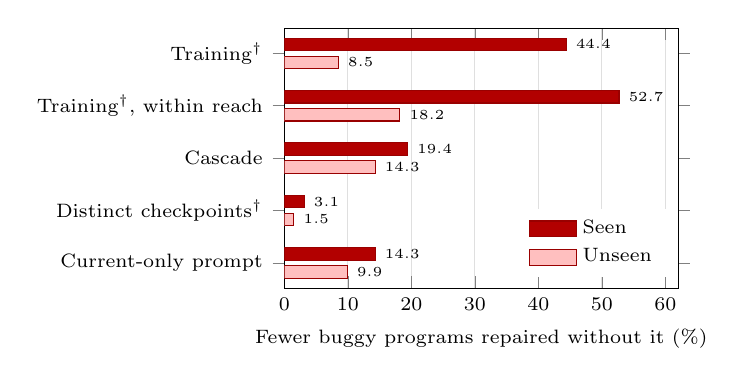
\begin{tikzpicture}
\begin{axis}[xbar, scale only axis, width=5.0cm, height=3.3cm, bar width=4.5pt, enlarge y limits=0.12,
 symbolic y coords={current,distinct,cascade,reach,training}, ytick={current,distinct,cascade,reach,training},
 yticklabels={{Current-only prompt}, {Distinct checkpoints\(^\dagger\)}, Cascade, {Training\(^\dagger\), within reach}, {Training\(^\dagger\)}}, y tick label style={font=\scriptsize},
 xmin=0, xmax=62, xtick={0,10,20,30,40,50,60}, x tick label style={font=\scriptsize}, xlabel={Fewer buggy programs repaired without it (\%)}, xlabel style={font=\scriptsize},
 xmajorgrids, grid style={gray!25}, nodes near coords={\pgfmathprintnumber[fixed, fixed zerofill, precision=1]{\pgfplotspointmeta}}, every node near coord/.append style={font=\tiny, anchor=west},
 area legend, reverse legend, legend cell align=left, legend style={font=\scriptsize, at={(0.97,0.04)}, anchor=south east}]
% rows:ablation
\addplot[fill=red!25, draw=red!60!black] coordinates {(8.5,training) (18.2,reach) (14.3,cascade) (1.5,distinct) (9.9,current)};
\addplot[fill=red!70!black, draw=red!60!black] coordinates {(44.4,training) (52.7,reach) (19.4,cascade) (3.1,distinct) (14.3,current)};
% end rows
\legend{Unseen, Seen}
\end{axis}
\end{tikzpicture}%
\caption{Fewer buggy programs repaired without each design choice}
\label{fig:ablation}
\end{figure}

% 학습을 제거하면 버기 프로그램을 Seen에서 44.4\%, Unseen에서 8.5\% 더 적게 수리했고, reach 안에서는 52.7\%와 18.2\% 더 적게 수리했다. cascade를 checkpoint 하나로 줄이면 19.4\%와 14.3\% 더 적게 수리했다. 서로 다른 세 checkpoint 대신 한 checkpoint에서 후보 세 개를 뽑으면 3.1\%와 1.5\% 더 적게 수리했다. 학생의 이전 제출을 prompt에 덧붙이면 14.3\%와 9.9\% 더 적게 수리했다. 따라서 네 선택은 각각 Seen과 Unseen 모두에서 수리율을 높였다.
Removing training repaired 44.4\% fewer buggy programs on Seen and 8.5\% fewer on Unseen, and 52.7\% and 18.2\% fewer within reach. Reducing the cascade to one checkpoint repaired 19.4\% and 14.3\% fewer. Drawing three candidates from one checkpoint instead of three distinct ones repaired 3.1\% and 1.5\% fewer. Adding the student's earlier submissions to the prompt repaired 14.3\% and 9.9\% fewer. Hence, each of the four choices raised the repair rate on both Seen and Unseen.

\begin{table}[h]
\caption{Repair rate, within-reach repair rate, and retention (\%) by target rule}
\label{tab:targets}
\centering\scriptsize
\setlength{\tabcolsep}{2.5pt}
\begin{tabular}{l|rrr|rrr|rrr|rrr}
\toprule
 & \multicolumn{3}{c|}{RR} & \multicolumn{3}{c|}{Within-reach RR} & \multicolumn{3}{c|}{Tokens} & \multicolumn{3}{c}{Lines} \\
 & A & S & P & A & S & P & A & S & P & A & S & P \\
\midrule
% rows:targets
Seen & 53.2 & 48.6 & 34.0 & 34.5 & 33.3 & 27.9 & 88.0 & 89.4 & 93.5 & 72.4 & 75.3 & 80.9 \\
Unseen & 76.8 & 74.8 & 65.6 & 44.8 & 45.2 & 48.8 & 81.2 & 84.1 & 87.8 & 57.8 & 62.2 & 68.3 \\
% end rows
\bottomrule
\end{tabular}
\end{table}

% \noindent\textbf{Target rule.} target 규칙만의 효과를 보기 위해, 우리는 Answer와 Progress의 target이 서로 다른 Seen 학습 예제 7,389개에서 현재 제출만 담은 prompt는 그대로 두고 target만 바꾸어 Answer, Strict, Progress마다 checkpoint 세 개를 학습했다. Strict의 target은 현재 제출보다 덜 심각한 verdict를 받은 다음 제출이며, 이 예제의 57.6\%에서 Answer의 target과 같다. Table~\ref{tab:targets}은 세 checkpoint를 cascade로 실행한 Answer(A), Strict(S), Progress(P)의 RR과 reach 안 수리율, 그리고 세 규칙이 모두 수리한 버기 프로그램에서의 retention을 보인다. Progress의 patch는 Answer의 patch보다 학생의 token을 Seen에서 6.3\%, Unseen에서 8.1\% 더 많이, 줄을 11.9\%와 18.3\% 더 많이 남겼다. Progress target은 학생이 다음으로 앞으로 나아간 제출인 반면, Answer target은 accepted 프로그램으로서 다른 접근을 택할 수 있기 때문이다(Figure~\ref{fig:example}에서 TED 3 대 22).
\noindent\textbf{Target rule.} To isolate the target rule, we trained three checkpoints each of Answer, Strict, and Progress on the 7,389 Seen training examples whose Answer and Progress targets differ, keeping the current-only prompts and changing only the target. A Strict target is the next submission with a less severe verdict than the current one, and it equals the Answer target on 57.6\% of these examples. Table~\ref{tab:targets} lists the RR and within-reach repair rate of Answer (A), Strict (S), and Progress (P), each running its three checkpoints as a cascade, and their retention on the buggy programs that all three rules repair. The patches of Progress kept 6.3\% more of the student's tokens than those of Answer on Seen and 8.1\% more on Unseen, and 11.9\% and 18.3\% more of the lines. This is because a Progress target is the student's next forward submission, whereas an Answer target is the accepted program, which can take a different approach (a TED of 3 against 22 in Figure~\ref{fig:example}).

% 그 대가로 Progress는 Answer보다 버기 프로그램을 Seen에서 36.0\%, Unseen에서 14.6\% 더 적게 수리했는데, Answer target은 모두 accepted 제출인 반면 Progress target은 아직 통과하지 못한 개선이기 때문이다. reach 안 수리율에서는 Progress가 Seen에서 19.2\% 더 낮고 Unseen에서 8.9\% 더 높았는데, Progress 수리의 82.0\%와 74.4\%가 reach 안에 있어 Answer의 64.9\%와 58.3\%보다 높았기 때문이다. Strict는 Answer보다 버기 프로그램을 Seen에서 8.5\%, Unseen에서 2.6\% 더 적게 수리했지만, 학생의 token을 1.6\%와 3.5\% 더 많이 남겼다. 따라서 target 규칙은 수리율과 retention을 맞바꾸었으며, Seen과 Unseen 모두에서 수리율은 Answer, Strict, Progress 순으로 낮아지고 retention은 그 순으로 높아졌다.
In exchange, Progress repaired 36.0\% fewer buggy programs than Answer on Seen and 14.6\% fewer on Unseen, because every Answer target is an accepted submission, whereas the Progress targets are improvements that do not yet pass. In within-reach repair rate, Progress was 19.2\% lower on Seen and 8.9\% higher on Unseen, because 82.0\% and 74.4\% of its repairs lay within reach, against 64.9\% and 58.3\% of Answer's. Strict repaired 8.5\% fewer buggy programs than Answer on Seen and 2.6\% fewer on Unseen, but its patches kept 1.6\% and 3.5\% more of the student's tokens. Hence, the target rule traded repair rate for retention, and on both Seen and Unseen the repair rate fell and the retention rose in the order Answer, Strict, Progress.

\begin{table}[h]
\caption{Progress trained on the student's own and on another student's targets}
\label{tab:targetsource}
\centering\footnotesize
\begin{tabular}{l|rr|rr|rr}
\toprule
 & \multicolumn{2}{c|}{RR (\%)} & \multicolumn{2}{c|}{\shortstack{Within-reach\\RR (\%)}} & \multicolumn{2}{c}{Mean TED} \\
 & Own & Other & Own & Other & Own & Other \\
\midrule
% rows:targetsource
Seen & 50.4 & 54.7 & 21.6 & 11.9 & 47.6 & 63.7 \\
Unseen & 78.4 & 84.4 & 29.2 & 12.8 & 30.0 & 44.4 \\
% end rows
\bottomrule
\end{tabular}
\end{table}

% \noindent\textbf{Target source.} target의 출처만의 효과를 보기 위해, 우리는 Seen 문제 453개의 Progress 학습 예제 5,231개에서 현재 제출만 담은 prompt는 그대로 두고, 각 target을 같은 문제에 대한 다른 학생의 제출 가운데 실행 결과가 같고 현재 제출과의 token 차이가 원래 target과 가장 비슷한 제출로 바꾸어, 두 target마다 checkpoint 세 개를 학습했다. Table~\ref{tab:targetsource}는 학생 자신의 target(Own)과 다른 학생의 target(Other)으로 학습한 Progress의 RR과 reach 안 수리율, 그리고 둘 다 수리한 버기 프로그램에서의 평균 TED를 보인다. 다른 학생의 target으로 학습하면 버기 프로그램을 Seen에서 8.6\%, Unseen에서 7.7\% 더 많이 수리했지만, reach 안 수리율은 44.7\%와 56.2\% 더 낮았고, 둘 다 수리한 버기 프로그램에서 patch의 TED가 33.8\%와 48.0\% 더 컸다. 다른 학생의 제출은 실행 결과와 token 차이가 같더라도 현재 학생의 프로그램에서 출발하지 않기 때문이다. 따라서 patch를 학생의 reach 안에 머물게 한 것은 학생 자신의 trajectory에서 온 target이었다.
\noindent\textbf{Target source.} To isolate the source of the targets, we took the 5,231 Progress training examples of 453 Seen problems with current-only prompts, replaced each target with another student's submission to the same problem that has the same execution outcomes and whose token difference from the current submission is closest to that of the original target, and trained three checkpoints on each set of targets. Table~\ref{tab:targetsource} lists the RR and within-reach repair rate of Progress trained on the student's own targets (Own) and on another student's (Other), and the mean TED on the buggy programs both repair. With another student's targets, Progress repaired 8.6\% more buggy programs on Seen and 7.7\% more on Unseen, but its within-reach repair rate was 44.7\% and 56.2\% lower, and on the buggy programs both repair its patches had a 33.8\% and 48.0\% larger TED. This is because another student's submission does not start from the current student's program, even with the same execution outcomes and token difference. Hence, the targets from the student's own trajectory, rather than training on the same problems alone, kept the patches within the student's reach.

% 이 결과들은 학습, 서로 다른 checkpoint의 cascade, 현재 제출만 담은 prompt가 각각 \textsc{ZPDPatch}의 수리율을 높이고, target 규칙이 수리율과 retention을 맞바꾸며, patch를 학생의 reach 안에 머물게 하는 것은 학생 자신의 trajectory에서 온 target이라는 것을 보여 준다.
These results show that training, the cascade of distinct checkpoints, and current-only prompts each raise the repair rate of \textsc{ZPDPatch}, that the target rule trades repair rate for retention, and that what keeps the patches within the student's reach is the targets from the student's own trajectory.

\subsection{RQ4: Generality}
\label{sec:generality}

% RQ4에 답하기 위해, 우리는 checkpoint 하나와 cascade의 비교(RQ3의 \textsc{ZPDPatch}-Cascade)를 Qwen2.5-Coder-1.5B-Instruct~\cite{hui2024qwen2}를 base model로 하여, 그리고 학생이나 문제를 학습에서 제외한 Java에서 반복했다. 또한 RQ3의 target 규칙 비교를 학생을 학습에서 제외한 Java에서 반복했다.
To answer RQ4, we repeated the comparison of one checkpoint with the cascade (\textsc{ZPDPatch}-Cascade in RQ3) with Qwen2.5-Coder-1.5B-Instruct~\cite{hui2024qwen2} as the base model and on Java with students or problems held out of training. We also repeated the target-rule comparison of RQ3 on Java with students held out of training.

\begin{figure}[h]
\centering
\begin{minipage}[t]{0.6\columnwidth}\centering
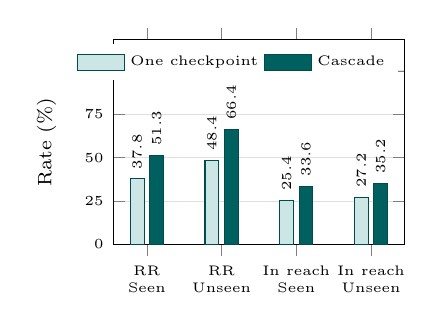
\begin{tikzpicture}
\begin{axis}[ybar, scale only axis, height=2.6cm, bar width=5pt, x tick label style={font=\tiny, align=center}, ymin=0, ymax=118, ytick={0,25,50,75,100}, y tick label style={font=\tiny}, ymajorgrids, grid style={gray!25}, nodes near coords={\pgfmathprintnumber[fixed, fixed zerofill, precision=1]{\pgfplotspointmeta}}, every node near coord/.append style={font=\tiny, rotate=90, anchor=west}, width=3.7cm, enlarge x limits=0.15,
 symbolic x coords={rrseen,rrunseen,reachseen,reachunseen}, xtick=data, xticklabels={{RR\\Seen}, {RR\\Unseen}, {In reach\\Seen}, {In reach\\Unseen}},
 ylabel={Rate (\%)}, ylabel style={font=\scriptsize}, legend columns=2, area legend, legend cell align=left, legend style={font=\tiny, at={(0.98,0.98)}, anchor=north east}]
% rows:generality15
\addplot[fill=teal!20, draw=teal!60!black] coordinates {(rrseen,37.8) (rrunseen,48.4) (reachseen,25.4) (reachunseen,27.2)};
\addplot[fill=teal!75!black, draw=teal!60!black] coordinates {(rrseen,51.3) (rrunseen,66.4) (reachseen,33.6) (reachunseen,35.2)};
% end rows
\legend{One checkpoint, Cascade}
\end{axis}
\end{tikzpicture}\\
{\footnotesize (a) 1.5B model}
\end{minipage}\hfill
\begin{minipage}[t]{0.38\columnwidth}\centering
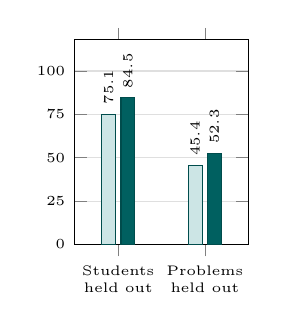
\begin{tikzpicture}
\begin{axis}[ybar, scale only axis, height=2.6cm, bar width=5pt, x tick label style={font=\tiny, align=center}, ymin=0, ymax=118, ytick={0,25,50,75,100}, y tick label style={font=\tiny}, ymajorgrids, grid style={gray!25}, nodes near coords={\pgfmathprintnumber[fixed, fixed zerofill, precision=1]{\pgfplotspointmeta}}, every node near coord/.append style={font=\tiny, rotate=90, anchor=west}, width=2.2cm, enlarge x limits=0.5,
 symbolic x coords={students,problems}, xtick=data, xticklabels={{Students\\held out}, {Problems\\held out}}]
% rows:generalityjava
\addplot[fill=teal!20, draw=teal!60!black] coordinates {(students,75.1) (problems,45.4)};
\addplot[fill=teal!75!black, draw=teal!60!black] coordinates {(students,84.5) (problems,52.3)};
% end rows
\end{axis}
\end{tikzpicture}\\
{\footnotesize (b) Java}
\end{minipage}
\caption{Repair rate and within-reach repair rate of one checkpoint and the cascade by setting}
\label{fig:generality}
\end{figure}

% Figure~\ref{fig:generality}는 checkpoint 하나(\textsc{ZPDPatch}-Cascade)와 cascade의 RR을 1.5B 모델(Figure~\ref{fig:generality}-(a))과 Java(Figure~\ref{fig:generality}-(b))에서 그리며, 1.5B 모델에서는 reach 안 수리율(In reach)도 그린다. 1.5B 모델에서 cascade는 checkpoint 하나보다 버기 프로그램을 Seen에서 35.5\%, Unseen에서 37.2\% 더 많이 수리했고, 학생의 reach 안에서는 32.4\%와 29.4\% 더 많이 수리했다. Java에서는 학생을 학습에서 제외했을 때 12.5\%, 문제를 학습에서 제외했을 때 15.2\% 더 많이 수리했다. 따라서 cascade의 이득은 더 작은 모델에서도, 다른 언어의 처음 보는 학생과 문제에서도 유지되었다.
Figure~\ref{fig:generality} plots the RR of one checkpoint (\textsc{ZPDPatch}-Cascade) and of the cascade with the 1.5B model (Figure~\ref{fig:generality}-(a)) and on Java (Figure~\ref{fig:generality}-(b)), and for the 1.5B model also the within-reach repair rate (In reach). With the 1.5B model, the cascade repaired 35.5\% more buggy programs than one checkpoint on Seen and 37.2\% more on Unseen, and 32.4\% and 29.4\% more within the student's reach. On Java, it repaired 12.5\% more with students held out of training and 15.2\% more with problems held out. Hence, the gain of the cascade held with a smaller model and on unseen students and problems in another language.

\begin{table}[h]
\caption{Repair rate and retention (\%) by target rule on Java}
\label{tab:javatargets}
\centering\footnotesize
\begin{tabular}{l|rrr}
\toprule
 & Answer & Strict & Progress \\
\midrule
% rows:javatargets
RR & 85.6 & 69.6 & 50.8 \\
Tokens & 90.9 & 95.6 & 95.8 \\
Lines & 86.1 & 90.3 & 91.2 \\
% end rows
\bottomrule
\end{tabular}
\end{table}

% Table~\ref{tab:javatargets}는 Java에서 각 target 규칙의 RR과 retention을 보이며, retention은 세 규칙이 모두 수리한 버기 프로그램에서 잰다. 각 규칙은 RQ3처럼 Answer와 Progress의 target이 서로 다른 학습 예제 600개로 학습했으므로, 모든 Answer 예제로 학습한 Figure~\ref{fig:generality}-(b)의 cascade와 RR이 다르다. Progress의 patch는 Answer의 patch보다 학생의 token을 5.4\%, 줄을 5.9\% 더 많이 남긴 반면, 버기 프로그램을 40.6\% 더 적게 수리했다. Strict는 Answer보다 버기 프로그램을 18.7\% 더 적게, Progress보다는 37.0\% 더 많이 수리했고, 그 patch는 Answer의 patch보다 token을 5.2\%, 줄을 4.8\% 더 많이 남겼다. 따라서 Java에서도 target 규칙은 Seen과 Unseen에서처럼 수리율과 retention을 맞바꾸었다.
Table~\ref{tab:javatargets} lists the RR and retention of each target rule on Java, with retention measured on the buggy programs that all three rules repair. As in RQ3, each rule was trained on the 600 training examples whose Answer and Progress targets differ, so its RR differs from that of the cascade in Figure~\ref{fig:generality}-(b), which was trained on all Answer examples. The patches of Progress kept 5.4\% more of the student's tokens and 5.9\% more of the lines than those of Answer, while Progress repaired 40.6\% fewer buggy programs. Strict repaired 18.7\% fewer buggy programs than Answer but 37.0\% more than Progress, and its patches kept 5.2\% more of the student's tokens and 4.8\% more of the lines than those of Answer. Hence, on Java as well, the target rule traded repair rate for retention as on Seen and Unseen.

% 이 결과들은 더 작은 모델에서도, 그리고 학생이나 문제를 학습에서 제외한 CS1 Java 과목에서도 checkpoint 세 개가 하나보다 더 많이 수리하며, Java에서도 target 규칙이 수리율과 retention을 맞바꾼다는 것을 보여 준다.
These results indicate that three checkpoints repair more than one with a smaller model as well as on a CS1 Java course with students or problems held out of training, and that the target rule trades repair rate for retention on Java as well.

\subsection{Threats to Validity}
% (1) 학습에 쓰인 문제에서 \textsc{ZPDPatch}는 버기 프로그램을 수리하는 대신 암기한 accepted 제출을 돌려줄 수 있다. 그러나 학생을 학습에서 제외한 RQ1 벤치마크에서 그 수리 583개 가운데 같은 문제의 학습용 accepted 제출과 같은 것은 하나도 없었다. (2) 기존 기법과의 차이는 target이 아니라 모델에서 올 수 있다. 그러나 \textsc{ZPDPatch}의 patch는 우리 base model을 쓰는 \textsc{LSGen}\textsubscript{Qwen}의 patch보다 TED가 60.9\% 작았고(RQ2), target만 다른 학생의 제출로 바꾸면 TED가 33.8--48.0\% 커졌다(RQ3). (3) 우리 데이터셋은 모든 유형의 과제를 다루지 못할 수 있다. 그러나 데이터셋은 Python과 Java 테스트 집합에 걸친 서로 다른 문제 403개의 버기 프로그램 3,000개 이상을 담아, 선행 기법들의 벤치마크~\cite{hu2019re,xie2024brafar,dai2026learner}보다 문제가 6.2--80.6배 많다. (4) 수리는 test suite를 통과할 뿐 모든 입력을 통과하는 것은 아니다~\cite{smith2015cure}. 그러나 생성한 입력 가운데 학생 자신의 accepted 프로그램이 통과하는 것만 세면, \textsc{ZPDPatch}의 plausible patch는 3.1\%가 실패하여 어느 기존 기법(3.4--6.5\%)보다 적었다.
(1) On problems used in training, \textsc{ZPDPatch} may return a memorized accepted submission instead of repairing the buggy program. However, on the RQ1 benchmark, whose students are held out of training, none of its 583 repairs equaled an accepted training submission of the same problem. (2) The difference from existing techniques may come from the model rather than from the targets. However, the patches of \textsc{ZPDPatch} had a 60.9\% smaller TED than those of \textsc{LSGen}\textsubscript{Qwen}, which uses our base model (RQ2), and replacing only the targets with another student's submissions made the TED 33.8--48.0\% larger (RQ3). (3) Our datasets may not cover every type of assignment. However, they hold over 3,000 buggy programs of 403 distinct problems across our Python and Java test sets, 6.2--80.6 times as many problems as the benchmarks of prior techniques~\cite{hu2019re,xie2024brafar,dai2026learner}. (4) A repair passes the test suite, not every input~\cite{smith2015cure}. However, on generated inputs that the student's own accepted program passes, 3.1\% of the plausible patches of \textsc{ZPDPatch} failed, fewer than for any existing technique (3.4--6.5\%).

\section{Related Work}
\label{sec:related}
% \noindent\textbf{Automated Feedback Generation for Programming Assignments.} 우리 연구는 학생의 프로그램을 수리하는 Automated Feedback Generation(AFG) 기법과 목표를 공유하며, 이 기법들은 수리를 정답 코드 쪽으로 이끄는 여러 방법을 발전시켜 왔다. Reference-driven 기법은 강사의 오류 모델로 탐색하거나~\cite{singh2013automated}, 같은 문제의 reference program을 군집화하거나~\cite{gulwani2018automated} 정렬하며~\cite{wang2018search,ahmed2022verifix}, \textsc{Qlose}~\cite{d2016qlose}는 patch와 학생의 프로그램 사이의 거리를 최소화하지만 정답 프로그램 쪽으로 그렇게 한다. Model-driven 기법은 과제 정보를 쓰는 transformer~\cite{heo2023referent}나 code infilling 모델~\cite{koutcheme2023automated}로 피드백을 생성한다. 우리가 비교하지 않는 model-driven 기법 가운데 \textsc{PyDex}는 더 이상 사용할 수 없는 Codex를 기반으로 하고~\cite{zhang2024pydex}, \textsc{Cref}는 튜터의 지도를 받으며~\cite{yang2024cref}, Phung 등은 문법 오류만 수리하며~\cite{phung2023generating}, \textsc{FastFixer}~\cite{liu2024fastfixer}와 \textsc{PaR}~\cite{zhao2026peer}는 C 과제에서만 평가되었다. 가장 가까운 \textsc{LSGen}~\cite{dai2026learner}과의 핵심 차이는, \textsc{LSGen}이 수리할 때 다른 학생들의 틀린 제출과 correct program의 쌍을 in-context 예시로 검색하는 반면, \textsc{ZPDPatch}는 학생 자신의 이후 제출과 Mine이 찾은 앞으로 나아간 걸음으로 fine-tune되고 수리할 때는 현재 제출만 읽는다는 점이다. Next-step hint는 과거 학생들의 경로로 만든 해답 공간에 제출을 투영하므로, 같은 위치에 있는 학생들은 같은 다음 걸음을 받으며~\cite{barnes2008toward,paassen2017continuous,piech2015autonomously,rivers2017data,price2017isnap}, 완전한 프로그램이 아니라 편집 하나나 자연어 메시지를 돌려준다~\cite{roest2024next}. tutoring system과 knowledge tracing은 관측 가능한 수행이나 상호작용 기록, 코드에서는 test case별 결과로부터 학습자의 현재 수준을 추정하고~\cite{murray2002toward,chounta2017grey,schulze2024beyond,corbett1994knowledge,piech2015deep,duan2025test}, 학생 코드 모델은 학생의 다음 제출~\cite{liu2022open}이나 단계적 편집~\cite{miroyan2025parastudent}을 실수까지 흉내 내 생성한다. 이들과 달리 \textsc{ZPDPatch}는 학생 크기의 걸음을 배우고, 현재 제출만 읽어 test suite를 모두 통과하거나 앞으로 나아간 완전한 프로그램을 돌려준다.
\noindent\textbf{Automated Feedback Generation for Programming Assignments.} Our work shares a common goal with Automated Feedback Generation (AFG) techniques that repair a student's program, which have developed many ways to steer the repair toward correct code. Reference-driven techniques search with an instructor's error model~\cite{singh2013automated}, or cluster~\cite{gulwani2018automated} or align~\cite{wang2018search,ahmed2022verifix} the reference programs of the same problem, and \textsc{Qlose}~\cite{d2016qlose} also minimizes a patch's distance to the student's program, but toward a correct program. Model-driven techniques generate feedback with a transformer given assignment information~\cite{heo2023referent} or with code-infilling models~\cite{koutcheme2023automated}. Among the model-driven techniques we do not compare with, \textsc{PyDex} builds on Codex, which is no longer available~\cite{zhang2024pydex}, \textsc{Cref} takes a tutor's guidance~\cite{yang2024cref}, Phung et al. repair only syntax errors~\cite{phung2023generating}, and \textsc{FastFixer}~\cite{liu2024fastfixer} and \textsc{PaR}~\cite{zhao2026peer} were evaluated only on C assignments. The key difference from the closest technique, \textsc{LSGen}~\cite{dai2026learner}, is that \textsc{LSGen} retrieves other students' pairs of wrong submissions and correct programs as in-context examples at repair time, whereas \textsc{ZPDPatch} is fine-tuned on students' own later submissions, including the forward steps it mines, and reads only the current submission at repair time. Next-step hints project a submission onto a solution space built from past students' paths, so students at the same position receive the same next step~\cite{barnes2008toward,paassen2017continuous,piech2015autonomously,rivers2017data,price2017isnap}, as a single edit or a natural-language message~\cite{roest2024next}, not a complete program. Tutoring systems and knowledge tracing estimate the learner's current level from observable performance or interaction records, for code also per test case~\cite{murray2002toward,chounta2017grey,schulze2024beyond,corbett1994knowledge,piech2015deep,duan2025test}, and student-code models generate a student's next submission~\cite{liu2022open} or incremental edits~\cite{miroyan2025parastudent}, mistakes included. Unlike these, \textsc{ZPDPatch} learns student-sized steps and returns, from the current submission alone, a complete program that passes the test suite or moves forward.

% \noindent\textbf{Supervision for Program Repair.} 우리 연구는 target 프로그램을 향해 학습하거나 탐색하는 수리 기법과 관련되지만, target이 무엇이냐에서 다르다. 학생의 컴파일 오류에 대해 수리 모델은 컴파일되지 않는 제출과 그 학생의 다음 컴파일되는 제출의 쌍~\cite{ahmed2018compilation}, 문법적으로 올바른 제출~\cite{bhatia2018neuro}, 또는 정답 프로그램에 심은 오류~\cite{gupta2017deepfix,yasunaga2020graph}로부터 학습하므로, target은 컴파일되는 코드다. test case에서 실패하는 제출에 대해 이들은 정답 제출~\cite{pu2016sk_p}, 학생들이 그런 제출을 고치려고 한 편집~\cite{rolim2017learning}, 또는 수리 도구의 patch~\cite{koutcheme2023training}로부터 학습한다. 일반 Automated Program Repair(APR)는 개발자의 수리 쌍으로부터 학습하거나~\cite{tufano2019empirical,lutellier2020coconut}, 정답 코드를 일부러 망가뜨려 학습 쌍을 만들거나~\cite{yasunaga2021break,ye2022selfapr}, 학습 없이 언어 모델을 사용한다~\cite{xia2022less}. 어느 경우든 target은 정답 코드이며, 반드시 학생 자신의 코드인 것은 아니다. Search-based APR은 모든 test case를 통과하는 프로그램에 도달하기 위해, 통과한 test case에 가중치를 주거나~\cite{le2011genprog} patch 크기와 절충하여~\cite{yuan2018arja} 후보에 점수를 매기며, 프로그래밍 프로젝트의 평가에서는 test 생성 도구와 수리 도구가 정확성 판정에 정보를 주지만 여전히 결함 있는 제출을 많이 놓친다~\cite{gu2025can}. 반면 \textsc{ZPDPatch}는 test case에서 실패하는 제출에 대해 같은 학생의 이후 제출을 target으로 삼고, test case별 실행 결과를 정확성 판정이나 통과 개수가 아니라 학생 자신의 이전 제출에 대한 Pareto 지배로 비교하여, 틀린 제출이 앞으로 나아갔는지를 판단한다.
\noindent\textbf{Supervision for Program Repair.} Our work relates to repair techniques that learn or search toward a target program, but differs in what the target is. For students' compilation errors, repair models learn from a non-compiling submission paired with the student's next compiling one~\cite{ahmed2018compilation}, from syntactically correct submissions~\cite{bhatia2018neuro}, or from errors seeded into correct programs~\cite{gupta2017deepfix,yasunaga2020graph}, so the target is code that compiles. For submissions failing test cases, they learn from correct submissions~\cite{pu2016sk_p}, from the edits students made to fix such submissions~\cite{rolim2017learning}, or from a repair tool's patches~\cite{koutcheme2023training}. General Automated Program Repair (APR) learns from developers' repair pairs~\cite{tufano2019empirical,lutellier2020coconut}, builds training pairs by breaking correct code on purpose~\cite{yasunaga2021break,ye2022selfapr}, or uses a language model without training~\cite{xia2022less}. In each case the target is correct code, not necessarily the student's own. Search-based APR scores a candidate by its passed test cases, weighted~\cite{le2011genprog} or traded off against patch size~\cite{yuan2018arja}, to reach a program that passes them all, and in assessing programming projects, test generation and repair tools inform correctness judgments but still miss many faulty submissions~\cite{gu2025can}. In contrast, for submissions that fail test cases, \textsc{ZPDPatch} takes as its target a later submission of the same student and compares test-case-wise outcomes, not to judge correctness or count passes but by Pareto dominance over the student's own earlier submission, to decide whether a wrong submission moved forward.

\section{Conclusion}
\label{sec:conclusion}
% 기존 Automated Feedback Generation 기법은 정답 프로그램을 목표로 삼으므로 그 patch가 학생의 가장 큰 걸음을 자주 넘지만, 학생은 한 걸음씩 앞으로 나아간다. 이 논문은 학생의 Zone of Proximal Development 안의 걸음을 돌려주는 trajectory-supervised repair 기법 \textsc{ZPDPatch}를 제시한다. \textsc{ZPDPatch}는 학생의 앞으로 나아간 걸음을 mine하고, 짝짓는 규칙마다 모델을 학습하며, 검증 프로그램을 함께 가장 많이 수리하는 모델들을 고른다. 실험 결과는 최신 기법과 비교해 \textsc{ZPDPatch}의 수리 가운데 학생의 reach 안에 드는 비율이 더 크고, 그 patch가 더 작고 학생의 code를 더 많이 남기며 학생의 accepted 프로그램과 더 자주 일치하고, 그 앞으로 나아간 걸음이 학생 자신의 걸음을 닮았음을 보여 준다.
Existing Automated Feedback Generation techniques aim at a correct program, so their patches often exceed a student's largest step, whereas students move forward step by step. This paper presents \textsc{ZPDPatch}, a trajectory-supervised repair technique that returns steps within the student's Zone of Proximal Development. \textsc{ZPDPatch} mines students' forward steps, trains a model per pairing rule, and selects the models that together repair the most validation programs. Experimental results demonstrate that, against state-of-the-art techniques, a larger share of the repairs of \textsc{ZPDPatch} lies within the student's reach, its patches are smaller, keep more of the student's code, and more often match the student's accepted program, and its forward steps resemble the students' own.

\bibliographystyle{IEEEtran}
\bibliography{references}
\end{document}
